\documentclass[11pt]{aghdpl}
% \documentclass[en,11pt]{aghdpl}  % praca w języku angielskim

% Lista wszystkich języków stanowiących języki pozycji bibliograficznych użytych w pracy.
% (Zgodnie z zasadami tworzenia bibliografii każda pozycja powinna zostać utworzona zgodnie z zasadami języka, w którym dana publikacja została napisana.)
\usepackage[english,polish]{babel}

% Użyj polskiego łamania wyrazów (zamiast domyślnego angielskiego).
\usepackage{polski}

\usepackage[utf8]{inputenc}

% dodatkowe pakiety

\usepackage{mathtools}
\usepackage{amsfonts}
\usepackage{amsmath}
\usepackage{amsthm}

% --- < bibliografia > ---

\usepackage[
style=numeric,
sorting=none,
%
% Zastosuj styl wpisu bibliograficznego właściwy językowi publikacji.
language=autobib,
autolang=other,
% Zapisuj datę dostępu do strony WWW w formacie RRRR-MM-DD.
urldate=iso8601,
% Nie dodawaj numerów stron, na których występuje cytowanie.
backref=false,
% Podawaj ISBN.
isbn=true,
% Nie podawaj URL-i, o ile nie jest to konieczne.
url=false,
%
% Ustawienia związane z polskimi normami dla bibliografii.
maxbibnames=3,
% Jeżeli używamy BibTeXa:
backend=bibtex
]{biblatex}

\usepackage{csquotes}
% Ponieważ `csquotes` nie posiada polskiego stylu, można skorzystać z mocno zbliżonego stylu chorwackiego.
\DeclareQuoteAlias{croatian}{polish}

\addbibresource{bibliografia.bib}

% Nie wyświetlaj wybranych pól.
%\AtEveryBibitem{\clearfield{note}}


% ------------------------
% --- < listingi > ---

% Użyj czcionki kroju Courier.
\usepackage{courier}

\usepackage{listings}
\lstloadlanguages{TeX}

\lstset{
	literate={ą}{{\k{a}}}1
           {ć}{{\'c}}1
           {ę}{{\k{e}}}1
           {ó}{{\'o}}1
           {ń}{{\'n}}1
           {ł}{{\l{}}}1
           {ś}{{\'s}}1
           {ź}{{\'z}}1
           {ż}{{\.z}}1
           {Ą}{{\k{A}}}1
           {Ć}{{\'C}}1
           {Ę}{{\k{E}}}1
           {Ó}{{\'O}}1
           {Ń}{{\'N}}1
           {Ł}{{\L{}}}1
           {Ś}{{\'S}}1
           {Ź}{{\'Z}}1
           {Ż}{{\.Z}}1,
	basicstyle=\footnotesize\ttfamily,
}

% ------------------------

\AtBeginDocument{
	\renewcommand{\tablename}{Tabela}
	\renewcommand{\figurename}{Rys.}
}

% ------------------------
% --- < tabele > ---

\usepackage{array}
\usepackage{tabularx}
\usepackage{multirow}
\usepackage{booktabs}
\usepackage{makecell}
\usepackage[flushleft]{threeparttable}

% defines the X column to use m (\parbox[c]) instead of p (`parbox[t]`)
\newcolumntype{C}[1]{>{\hsize=#1\hsize\centering\arraybackslash}X}


%---------------------------------------------------------------------------

\author{Kamil Osuch}
\shortauthor{K. Osuch}

%\titlePL{Przygotowanie bardzo długiej i pasjonującej pracy dyplomowej w~systemie~\LaTeX}
%\titleEN{Preparation of a very long and fascinating bachelor or master thesis in \LaTeX}

\titlePL{Opracowanie prototypu interfejsu dla gier wykorzystujących pętlę afektywną}
\titleEN{Development of a prototype interface for games based on the affective loop}


\shorttitlePL{Przygotowanie pracy dyplomowej w~systemie \LaTeX} % skrócona wersja tytułu jeśli jest bardzo długi
\shorttitleEN{Preparation of a long and fascinating thesis in \LaTeX}

\thesistype{Praca dyplomowa magisterska}
%\thesistype{Master of Science Thesis}

\supervisor{dr hab. Grzegorz Jacek Nalepa}
%\supervisor{Marcin Szpyrka PhD, DSc}

\degreeprogramme{Informatyka}
%\degreeprogramme{Computer Science}

\date{2015}

\department{Katedra Informatyki Stosowanej}
%\department{Department of Applied Computer Science}

\faculty{Wydział Elektrotechniki, Automatyki,\protect\\[-1mm] Informatyki i Inżynierii Biomedycznej}
%\faculty{Faculty of Electrical Engineering, Automatics, Computer Science and Biomedical Engineering}

\acknowledgements{Serdecznie dziękuję \dots tu ciąg dalszych podziękowań np. dla promotora, żony, sąsiada itp.}


\setlength{\cftsecnumwidth}{10mm}

%---------------------------------------------------------------------------
\setcounter{secnumdepth}{4}
\brokenpenalty=10000\relax

\begin{document}

\titlepages

% Ponowne zdefiniowanie stylu `plain`, aby usunąć numer strony z pierwszej strony spisu treści i poszczególnych rozdziałów.
\fancypagestyle{plain}
{
	% Usuń nagłówek i stopkę
	\fancyhf{}
	% Usuń linie.
	\renewcommand{\headrulewidth}{0pt}
	\renewcommand{\footrulewidth}{0pt}
}

\setcounter{tocdepth}{2}
\tableofcontents
\clearpage

\chapter{Wstęp}
\label{cha:wstep}
W ciągu ostatnich lat pojęcie sztucznej inteligencji przestało być tylko fenomenem, który dla większości społeczeństwa istniał pod postacią filmów lub powieści dotyczących maszyn posiadających świadomość. Od tamtego momentu człowiek zaczął znajdować zastosowanie sztucznej inteligencji w coraz większej liczbie dziedzin. Od maszyn przetwarzających w sposób automatyczny ogromne ilości informacji, aż po systemy gromadzące dane dotyczące użytkowników i~na ich podstawie generujące reguły, dzięki którym możliwe jest znalezienie rozwiązań i~porad dopasowanych do danego użytkownika.

Najistotniejszy jest w tym fakt, że człowiek otacza się sztuczną inteligencją, nawet tego nie zauważając. Systemy rekomendujące, dopasowujące produkty z każdej tematyki do preferencji użytkowników~\cite{Gomez-Uribe:2015:NRS:2869770.2843948}, urządzenia nasobne monitorujące nasz stan zdrowia dzięki pomiarom parametrów życiowych i~zbieraniu informacji na temat naszych nawyków~\cite{wearable_computing_amft}, czy coraz popularniejsze systemy autonomicznej jazdy~\cite{dikmen_tesla_autopilot}. Sztuczna inteligencja z dnia na dzień coraz bardziej wnika w każdy aspekt życia człowieka. 

Jednym z elementów, który odgrywa ważną rolę w życiu człowieka, a który coraz mocniej oparty jest o sztuczną inteligencję, są gry komputerowe.  Choć początkowo były one traktowane wyłącznie jako rozrywka, to dziś coraz częściej są określane nawet jako pewna forma nauki konkretnych umiejętności~\cite{oberdorfer_develop_your_strengths_by_gaming}. Przykładem mogą być tutaj gatunek gier strategicznych, które uczą taktyki i~zarządzania, a także gry logiczne pozwalające na rozwój logicznego myślenia. Warto tutaj wspomnieć także o grach poważnych~\cite{serious_games_michael_chen}, które nie skupiają się na aspektach rozrywkowych, a bardziej są formą edukacji i~szkoleń przedstawionych w formie interaktywnej symulacji.

Pojęciem, które jest coraz szerzej widoczne w kontekście sztucznej inteligencji związanej przede wszystkim z tematyką komunikacji człowiek-komputer jest informatyka afektywna. Chociaż samo pojęcie istnieje już od ponad 20 lat~\cite{Picard:1997:AC:265013}, to dopiero w ciągu kilku ostatnich badania w tej tematyce stały się popularne~\cite{gartner_hype_cycles_2018}. Początkowo główną ideą tej dziedziny były systemy zbierające i~analizujące dane na temat stanów emocjonalnych użytkowników. Ponieważ emocje nie mogą być kontrolowane poprzez działania człowieka, a jednocześnie można je opisać między innymi przy pomocy zmian fizjologicznych w ludzkim ciele, wykorzystanie informatyki afektywnej w systemach inteligentnych takich jak aplikacje rekomendujące czy systemy badające stan zdrowotny użytkowników pozwala na zwiększenie ich skuteczności działania.

W podobny sposób powstała próba powiązania dziedziny informatyki afektywnej z grami komputerowymi, tworząc nowy rodzaj gier, nazywanych grami afektywnymi. Główną ich ideą jest pomiar stanów emocjonalnych wywoływanych na użytkowniku w trakcie rozgrywki oraz dostosowywanie gry w czasie rzeczywistym do odczytanych reakcji gracza, tak aby zwiększyć doznania płynące z gry~\cite{kotsia_affective_gaming}. Dzięki temu każda gra może zostać w pewien sposób spersonalizowana na podstawie indywidualnych cech użytkownika. 

Celem pracy jest opracowanie prototypu dwuczęściowego interfejsu umożliwiającego pomiar sygnałów pozwalających na określenie zmian stanów emocjonalnych gracza. Interfejs ma posłużyć do opracowania prototypów gier zawierających pętlę afektywną. W skład interfejsu będą wchodzić:
\begin{itemize}
	\item zbiór urządzeń umożliwiających pomiary sygnałów wykorzystanych do określenia zmian emocji gracza
	\item moduł przygotowany w środowisku do tworzenia gier, który na podstawie zgromadzonych z urządzeń pomiarowych sygnałów będzie określał stan emocjonalny i~zachowania użytkownika
\end{itemize}
Ważnym elementem pracy jest stworzenie gry zawierającej pętlę afektywną~\cite{affective_loop_experiences}, która będzie wykorzystywała przygotowany interfejs. Po wykryciu zachowań oraz zmian stanów emocjonalnych użytkownika, stan gry jest aktualizowany.

Niniejsza praca składa się z 8 rozdziałów. W rozdziale \ref{cha:affectiveComputing} zostały przedstawione podstawy teoretyczne dotyczące informatyki afektywnej. Szczególny nacisk położono na tematykę gier afektywnych, przedstawiając wybrane istniejące rozwiązania, problemy i~kierunki badań z tego zakresu. Rozdział \ref{cha:specyfikacja} zawiera przedstawienie oraz analizę dostępnych sprzętowych platform pomiarowych, możliwych mechanizmów wnioskowania oraz narzędzi wykorzystywanych do budowy gier komputerowych. Ważnym elementem jest przedstawienie wad i~zalet każdego z rozwiązań w kontekście tematyki pracy. Rozdział \ref{cha:architektura} jest podsumowaniem analizy platform sprzętowych z poprzedniego rozdziału. Przedstawione tu zostały podstawowe założenia, jakie powinny być spełnione przez wybraną grupę urządzeń pomiarowych, a także definiuje sprzęt wybrany podczas końcowej implementacji. W rozdziale \ref{cha:predykcja} opisany został proces budowy modelu do rozpoznawania emocji. Omówione zostały wybrane zbiory danych, sposób ich przetwarzania, oraz budowa i~wybór końcowego modelu na podstawie działania z dostępnymi danymi. Rozdział \ref{cha:implementacja} jest jedną z najistotniejszych części pracy. Przedstawiono w nim proces implementacji utworzonej gry komputerowej z pętlą afektywną. Skupiono się na opisie interfejsu łączącego rozwiązania wybrane w poprzednich rozdziałach i~sposobie jego wykorzystania wewnątrz gry. Następnie przedstawione zostały mechaniki pokazujące, w jaki sposób przygotowany moduł może wpłynąć na rozgrywkę tak, by sprzężenie zwrotne mogło zostać zamknięte. W rozdziale \ref{cha:badania} opisany został sposób ewaluacji stworzonego rozwiązania oraz charakterystyka i~proces przeprowadzonych eksperymentów. Ostatni rozdział stanowi podsumowanie niniejszej pracy. Zawiera wnioski dotyczące przygotowanego projektu, jego mocne i~słabe strony. Opisane zostały także możliwe kierunki dalszego rozwoju projektu. 

\chapter{Pierwszy dokument}
\label{cha:pierwszyDokument}

W rozdziale tym przedstawiono podstawowe informacje dotyczące struktury prostych plików \LaTeX a. Omówiono również metody kompilacji plików z zastosowaniem programów \emph{latex} oraz \emph{pdflatex}.

%---------------------------------------------------------------------------

\section{Struktura dokumentu}
\label{sec:strukturaDokumentu}

Plik \LaTeX owy jest plikiem tekstowym, który oprócz tekstu zawiera polecenia formatujące ten tekst (analogicznie do języka HTML). Plik składa się z dwóch części:
\begin{enumerate}%[1)]
\item Preambuły -- określającej klasę dokumentu oraz zawierającej m.in. polecenia dołączającej dodatkowe pakiety;

\item Części głównej -- zawierającej zasadniczą treść dokumentu.
\end{enumerate}


\begin{lstlisting}
\documentclass[a4paper,12pt]{article}      % preambuła
\usepackage[polish]{babel}
\usepackage[utf8]{inputenc}
\usepackage[T1]{fontenc}
\usepackage{times}

\begin{document}                           % część główna

\section{Sztuczne życie}

% treść
% ąśężźćńłóĘŚĄŻŹĆŃÓŁ

\end{document}
\end{lstlisting}

Nie ma żadnych przeciwskazań do tworzenia dokumentów w~\LaTeX u w~języku polskim. Plik źródłowy jest zwykłym plikiem tekstowym i~do jego przygotowania można użyć dowolnego edytora tekstów, a~polskie znaki wprowadzać używając prawego klawisza \texttt{Alt}. Jeżeli po kompilacji dokumentu polskie znaki nie są wyświetlane poprawnie, to na 95\% źle określono sposób kodowania znaków (należy zmienić opcje wykorzystywanych pakietów).


%---------------------------------------------------------------------------

\section{Kompilacja}
\label{sec:kompilacja}


Załóżmy, że przygotowany przez nas dokument zapisany jest w pliku \texttt{test.tex}. Kolejno wykonane poniższe polecenia (pod warunkiem, że w pierwszym przypadku nie wykryto błędów i kompilacja zakończyła się sukcesem) pozwalają uzyskać nasz dokument w formacie pdf:
\begin{lstlisting}
latex test.tex
dvips test.dvi -o test.ps
ps2pdf test.ps
\end{lstlisting}
%
lub za pomocą PDF\LaTeX:
\begin{lstlisting}
pdflatex test.tex
\end{lstlisting}

Przy pierwszej kompilacji po zmiane tekstu, dodaniu nowych etykiet itp., \LaTeX~tworzy sobie spis rozdziałów, obrazków, tabel itp., a dopiero przy następnej kompilacji korzysta z tych informacji.

W pierwszym przypadku rysunki powinny być przygotowane w~formacie eps, a~w~drugim w~formacie pdf. Ponadto, jeżeli używamy polecenia \texttt{pdflatex test.tex} można wstawiać grafikę bitową (np. w formacie jpg).



%---------------------------------------------------------------------------

\section{Narzędzia}
\label{sec:narzedzia}


Do przygotowania pliku źródłowego może zostać wykorzystany dowolny edytor tekstowy. Niektóre edytory, np. GEdit, mają wbudowane moduły ułatwiające składanie tekstów w LaTeXu (kolorowanie składni, skrypty kompilacji, itp.).

Jednym z bardziej znanych środowisk do składania dokumentów  \LaTeX a jest {\em TeXstudio}, oferujące kompletne środowisko pracy. Zobacz: \url{http://www.texstudio.org}


Bardzo dobrym środowiskiem jest również edytor gEdit z wtyczką obsługującą \LaTeX a. Jest to standardowy edytor środowiska Gnome. Po instalacji wtyczki obsługującej \LaTeX~ zamienia się w wygodne i szybkie środowisko pracy.

\textbf{Dla testu łamania stron powtórzenia powyższego tekstu.}


Do przygotowania pliku źródłowego może zostać wykorzystany dowolny edytor tekstowy. Niektóre edytory, np. GEdit, mają wbudowane moduły ułatwiające składanie tekstów w LaTeXu (kolorowanie składni, skrypty kompilacji, itp.).
Jednym z bardziej znanych środowisk do składania dokumentów  \LaTeX a jest {\em TeXstudio}, oferujące kompletne środowisko pracy. Zobacz: \url{http://www.texstudio.org}
Bardzo dobrym środowiskiem jest również edytor gEdit z wtyczką obsługującą \LaTeX a. Jest to standardowy edytor środowiska Gnome. Po instalacji wtyczki obsługującej \LaTeX~ zamienia się w wygodne i szybkie środowisko pracy.
Po instalacji wtyczki obsługującej \LaTeX~ zamienia się w wygodne i szybkie środowisko pracy.

Do przygotowania pliku źródłowego może zostać wykorzystany dowolny edytor tekstowy. Niektóre edytory, np. GEdit, mają wbudowane moduły ułatwiające składanie tekstów w LaTeXu (kolorowanie składni, skrypty kompilacji, itp. itd. itp.).
Jednym z bardziej znanych środowisk do składania dokumentów  \LaTeX a jest {\em TeXstudio}, oferujące kompletne środowisko pracy. Zobacz: \url{http://www.texstudio.org}
Bardzo dobrym środowiskiem jest również edytor gEdit z wtyczką obsługującą \LaTeX a. Jest to standardowy edytor środowiska Gnome. Po instalacji wtyczki obsługującej \LaTeX~ zamienia się w wygodne i szybkie środowisko pracy.

Do przygotowania pliku źródłowego może zostać wykorzystany dowolny edytor tekstowy. Niektóre edytory, np. GEdit, mają wbudowane moduły ułatwiające składanie tekstów w LaTeXu (kolorowanie składni, skrypty kompilacji, itp.).
Jednym z bardziej znanych środowisk do składania dokumentów  \LaTeX a jest {\em TeXstudio}, oferujące kompletne środowisko pracy. Zobacz: \url{http://www.texstudio.org}
Bardzo dobrym środowiskiem jest również edytor gEdit z wtyczką obsługującą \LaTeX a. Jest to standardowy edytor środowiska Gnome. Po instalacji wtyczki obsługującej \LaTeX~ zamienia się w wygodne i szybkie środowisko pracy.

%---------------------------------------------------------------------------

\section{Przygotowanie dokumentu}
\label{sec:przygotowanieDokumentu}

Plik źródłowy \LaTeX a jest zwykłym plikiem tekstowym. Przygotowując plik
źródłowy warto wiedzieć o kilku szczegółach:

\begin{itemize}
\item
Poszczególne słowa oddzielamy spacjami, przy czym ilość spacji nie ma znaczenia.
Po kompilacji wielokrotne spacje i tak będą wyglądały jak pojedyncza spacja.
Aby uzyskać {\em twardą spację}, zamiast znaku spacji należy użyć znaku {\em
tyldy}.

\item
Znakiem końca akapitu jest pusta linia (ilość pusty linii nie ma znaczenia), a
nie znaki przejścia do nowej linii.

\item
\LaTeX~sam formatuje tekst. \textbf{Nie starajmy się go poprawiać}, chyba, że
naprawdę wiemy co robimy.
\end{itemize} 



\chapter{Specyfikacja komponentów interfejsu do rozpoznawania emocji}
\label{cha:specyfikacja}
Celem pracy jest opracowanie prototypu interfejsu umożliwiającego pomiar sygnałów pozwalających na określenie zmian stanów emocjonalnych gracza. W~związku z~tym na jeden z~elementów niniejszej pracy składa się przegląd możliwych rozwiązań użytych w~poszczególnych komponentach interfejsu. W~tym rozdziale skupiono się na przedstawieniu urządzeń do pomiaru sygnałów umożliwiających określenie stanu emocjonalnego użytkownika, mechanizmach wnioskowania, które mogą zostać użyte podczas budowania modelu do rozpoznawania emocji, oraz silnikach do budowy gier, przy pomocy których zostanie wykonany końcowy interfejs wraz z~grą.

\section{Platformy pomiarowe}
Odczyt sygnałów umożliwiających rozpoznawanie emocji jest jednym z~najważniejszych elementów w~pętli afektywnej. Obecnie dostępnych jest wiele platform umożliwiających wykonanie takich pomiarów i~można je podzielić na dwie główne kategorie: urządzenia służące do mierzenia reakcji fizjologicznych użytkownika oraz sprzęt umożliwiający odczyt sygnałów pośrednich, na podstawie których można określić stan użytkownika.

Na pierwszą grupę składają się między innymi platformy klasy medycznej umożliwiające dokładne pomiary z~ludzkiego ciała. Jednym z~takich urządzeń jest Neurobit Optima. Jest to przenośny sprzęt umożliwiający pomiar sygnałów takich jak praca serca, mózgu, ruchów mięśni, reakcji elektrodermalnej czy nawet temperatury skóry~\cite{neurobit_manual}. Ogromną zaletą Neurobit Optimy są wielofunkcyjne kanały pomiarowe, które użytkownik może dostosować do swoich potrzeb \cite{neurobit_manual}. Widocznym atutem z~perspektywy wykorzystania w~informatyce afektywnej jest gotowe oprogramowanie dostępne od producenta oraz wbudowany interfejs Bluetooth dający możliwość przenoszenia urządzenia. Pomiary z~Neurobit Optima charakteryzuje wysoka dokładność i~stabilność pomiarów. Podobnym do niego sprzętem jest NeXus-10, który także pozwala na pomiar pracy serca i~reakcji elektrodermalnej, posiada wbudowany interfejs Bluetooth oraz jest do niego dołączane gotowe oprogramowanie. Niestety ogromną wadą jest jego waga i~rozmiar wpływające negatywnie na wygodę podczas użytkowania. W~kontekście gier afektywnych potencjalną problemem urządzeń klasy medycznej może być także ich inwazyjność. Choć w~ciągu ostatnich lat środowisko sprzętowe wyszło daleko poza standardowy komputer czy konsole, to część z~graczy może nie zaakceptować platform kojarzonych z~medycyną jako części stanowiska do gier. Jednym z~problemów są tutaj szeroko wykorzystywane elektrody, które, choć umożliwiają dokładne pomiary sygnałów fizjologicznych, są kojarzone jednak głównie ze środowiskiem medycznym.

\begin{figure}
	\centering
	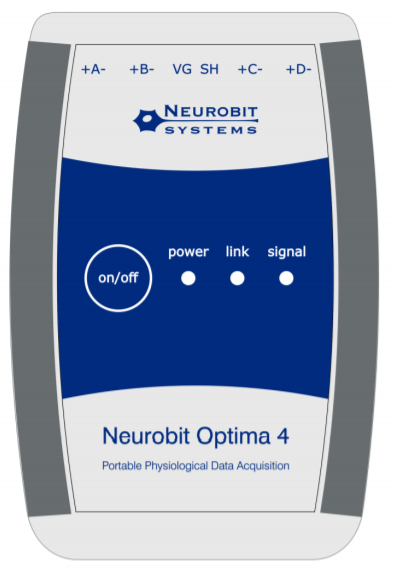
\includegraphics[width=0.3\linewidth]{images/neurobit_optima.png}
	\caption{Urządzenie Neurobit Optima, źródło: \cite{neurobit_manual}}
	\label{fig:neurobit}
\end{figure}

W kontekście platform do pomiarów sygnałów fizjologicznych w~informatyce afektywnej można zauważyć wzrost zainteresowania urządzeniami nasobnymi~\cite{wearable_sensors_2018}. Ich wyraźną zaletą jest rozmiar i~przenośność, dzięki czemu ruchy użytkownika nie są w~żadnym stopniu ograniczone. Najbardziej rozpowszechnionym, a~jednocześnie jednym z~tańszych rozwiązań, są inteligentne opaski, takie jak Xiaomi Mi Band czy Microsoft Band~\cite{wearable_sensors_2018}. Oba z~wymienionych urządzeń posiadają wbudowany optyczny sensor pulsu~\cite{miband_manual,microsoft_band_factsheet}, drugie natomiast posiada także czujnik do pomiaru reakcji elektrodermalnej~\cite{microsoft_band_factsheet}. Inną, mniej popularną opaską, jest Empatica E4, która poza sensorami dostępnymi w~Xiaomi Mi Band i~Microsoft Band umożliwia pomiar temperatury skóry~\cite{empatica_manual}. Warto wspomnieć też o~wbudowanych w~urządzenia czujnikach ruchu używanych między innymi do zliczania kroków mogących posłużyć jako sygnał pośredni, na podstawie którego można wykryć poziom aktywności użytkownika. Niestety ogromną wadą inteligentnych opasek jest duża niedokładność pomiarów w~porównaniu do odczytów ze sprzętów klasy medycznej. Wskazania z~opasek charakteryzują się wartościami mocno odbiegającymi od tych wykonanych przy pomocy sprzętu medycznego~\cite{wearable_sensors_2018,accuracy_of_wearables_hr}.

Innymi platformami nasobnymi charakteryzującymi się większą dokładnością, do których często porównuje się odczyty z~innych urządzeń do pomiaru pracy serca~\cite{wearable_sensors_2018,accuracy_of_wearables_hr}, są monitory tętna Garmin HRM-Run oraz Polar H10. W~przeciwieństwie do optycznego sensora wbudowanego w~inteligentne opaski są one wyposażone w~suche elektrody zamontowane w~pasku zakładanym na klatkę piersiową\cite{polar_manual,garmin_manual}. Jest to rozwiązanie, które nie jest inwazyjne dla użytkownika, a~jednocześnie pozwala na dokładny pomiar pracy serca. Ważną zaletą obu rozwiązań jest nie tylko wsparcie dla standardu Bluetooth, ale także dla protokołu ANT+ wykorzystywanego w~coraz większej liczbie urządzeń do pomiarów aktywności użytkownika\footnote{\textit{https://www.thisisant.com/directory}}, do którego twórcy udostępniają również gotowe implementacje interfejsów do odczytywania pomiarów. Dzięki temu w~prosty sposób możliwe jest zbudowanie aplikacji interpretujących wysyłane dane.

Rozwiązaniem będącym pomostem między kosztownymi platformami medycznymi a~często niedokładnymi urządzeniami nasobnymi jest platforma BITalino (r)evolution kit~\cite{bitalino_documentation}. Jest to narzędzie modułowe, składające się z~płytki stanowiącej rdzeń urządzenia, do której mogą zostać podpięte oddzielne moduły do pomiarów sygnałów fizjologicznych (rys. \ref{fig:bitalino}). Na liście dostępnych sensorów znajdują się te odpowiadające za pomiar akcji serca, reakcji elektrodermalnej skóry, czynności ruchowej mięśni oraz aktywności mózgu. Każdy z~modułów może zostać podłączony do dowolnego kanału urządzenia, natomiast pomiary odbywają się poprzez podłączenie do drugiej strony modułów kabli, na których końcu znajdują się elektrody. Co więcej, poza modułami służącymi do pomiaru reakcji fizjologicznych użytkownika, na liście dostępnych segmentów znajdują się także akcelerometr, sensor światła, dioda LED, brzęczyk, oraz przycisk, które mogą posłużyć do odczytu pomiarów pośrednich czy informowania użytkownika o~zdarzeniach. Dzięki temu platforma BITalino może służyć nie tylko jako urządzenie wykorzystywane do pomiarów, ale również do interakcji z~grą. Bardzo dużą zaletą BITalino z~perspektywy informatyki afektywnej jest dostępność narzędzi przygotowanych przez twórców, a~także ogromna ilość interfejsów do komunikacji z~urządzeniem. Twórcy na swojej stronie udostępniają biblioteki dla wielu popularnych języków programowania takich jak Python, C\# czy Java oraz konkretne implementacje z~przykładami dla środowisk takich jak silnik do gier Unity. Dodatkowym plusem jest fakt, że większość tych rozwiązań jest oprogramowaniem otwartym, w~związku z~czym mogą być one rozszerzane i~naprawiane przez społeczność korzystającą z~platformy.

\begin{figure}
	\centering
	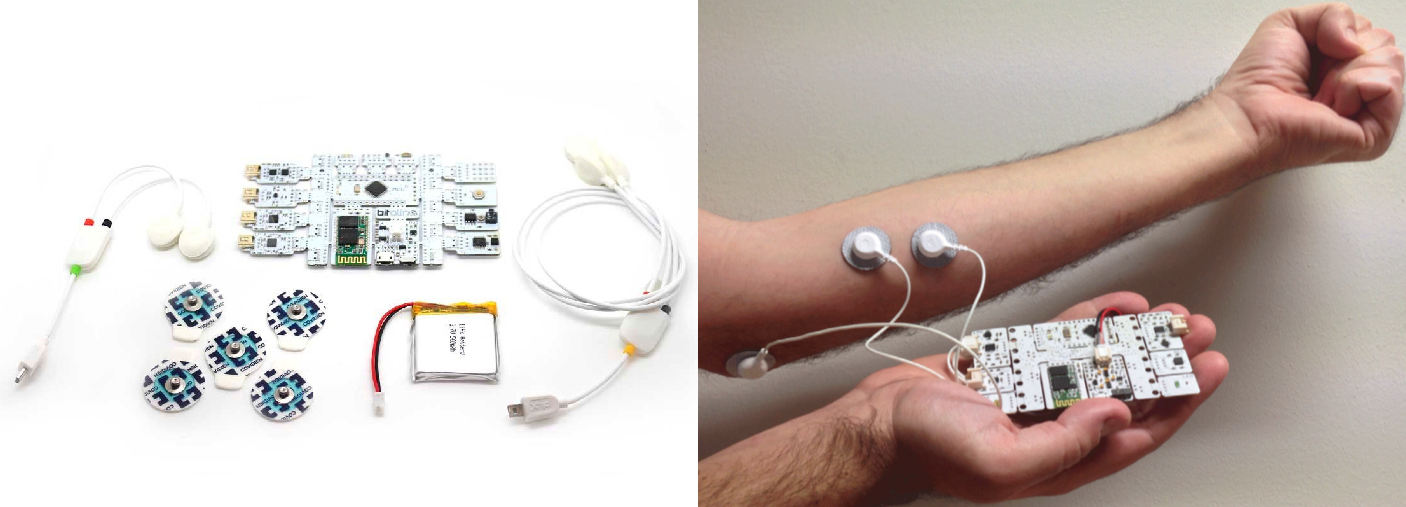
\includegraphics[width=0.9\linewidth]{images/bitalino_emg.png}
	\caption{BITalino (r)evolution kit oraz przykład podłączenia sensora do pomiaru ruchu mięśni, źródło: \cite{neurobit_manual}}
	\label{fig:bitalino}
\end{figure}

Do wspomnianej na początku drugiej kategorii urządzeń, z~których możliwe jest odczytanie sygnałów pośrednich wykorzystanych do określenia stanu użytkownika, można przede wszystkim zaliczyć sprzęty wykorzystywane przez graczy. Mowa tutaj między innymi o~myszkach, klawiaturach czy padach, z~których możliwe jest odczytanie intensywności kliknięć lub odczyt szybkości poruszania myszką na podstawie jej pozycji na ekranie~\cite{measuring_emotion_from_gamepad}. Szczególną uwagę należy poświęcić kontrolerowi DualShock 4~od firmy Sony, który w~przeciwieństwie do większości spopularyzowanych kontrolerów do gier posiada wbudowany akcelerometr oraz żyroskop, które mogą posłużyć jako dodatkowe źródło informacji do określenia stanu emocjonalnego użytkownika~\cite{dualshock_specification}. Niestety ze względu na umowy licencyjne oprogramowanie umożliwiające odczyt tych parametrów z~pada, jest płatne, co można zaliczyć jako wadę tego rozwiązania z~perspektywy twórcy aplikacji wykorzystującej funkcjonalności DualShocka.

\section{Możliwe mechanizmy do rozpoznawania emocji}
Aby określić emocje występujące u użytkownika na podstawie danych zebranych przy pomocy wybranych urządzeń, należy zaimplementować mechanizm sztucznej inteligencji, który jak najlepiej będzie umieć określić stan emocjonalny gracza. 

Poniżej przedstawiono i~opisano kilka wybranych metod wnioskowania, które mogłyby posłużyć jako algorytmy do modelu rozpoznającego stan emocjonalny użytkownika na podstawie zebranych danych fizjologicznych.

\subsection{Lasy losowe}
Lasy losowe są metodą uczenia maszynowego, która polega na zbudowaniu wielu drzew decyzyjnych, wykonaniu na nich klasyfikacji, a~następnie wybraniu klasy poprzez zasadę większości (rys. \ref{fig:random_forest}). Każde takie drzewo składa się z~wierzchołków, z~których wewnętrzne, nazywane węzłami, zawierają pytania i~warunki dotyczące sprawdzanych cech, natomiast zewnętrzne wierzchołki nazywane liśćmi zawierają decyzję o~klasyfikacji obiektów. Z~każdego węzła wychodzi tyle gałęzi, ile jest możliwych wyników warunku sprawdzanego na danym węźle.

Dla każdego z~drzew decyzyjnych wybierany jest podzbiór wejściowego zbioru danych za pomocą metody bootstrap, polegającej na losowaniu ze zwracaniem elementów z~podanego zbioru~\cite{flach_2012}. Liczność podzbiorów jest taka sama jak wejściowego zbioru danych, co oznacza, że niektóre elementy mogą znaleźć się w~nich więcej niż raz, a~inne w~ogóle nie zostaną uwzględnione. Dla każdego z~drzew wybierany jest także podzbiór cech, które będą brane pod uwagę przy tworzeniu wierzchołków drzewa. W~każdym węźle podział jest wybierany na podstawie tego, jak wiele informacji na temat wyboru klasy można uzyskać nam wybrany podzbiór cech.

\begin{figure}
	\centering
	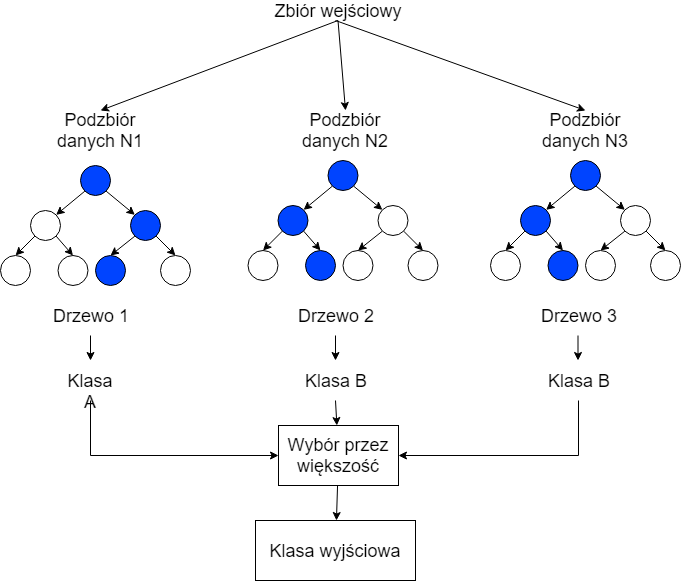
\includegraphics[width=0.7\linewidth]{images/random_forest.png}
	\caption{Uproszczony przykład działania metody lasów losowych}
	\label{fig:random_forest}
\end{figure}

\subsection{Drzewa ekstremalnie losowe} 
Metoda ta jest bardzo podobna do lasów losowych, z~dwoma istotnymi różnicami. Pierwszą jest brak tworzenia podzbiorów trenujących dla drzew. Każde z~nich jest uczone na tym samym zbiorze danych. Drugą różnicą jest sposób wyboru punktu podziału, który jest zupełnie losowy. Taka metoda zapewnia dużo mniejszy koszt obliczeń w~porównaniu do lasów losowych, ponieważ nie tracimy czasu na sprawdzenie, który z~podziałów daje najlepsze rezultaty.

\subsection{Maszyna z~wektorem wspierającym} 
Jest to metoda wykorzystywana głównie w~przypadku klasyfikacji. Głównym celem jest znalezienie linii lub hiperpłaszczyzny, która podzieli badany zbiór danych na dwie różne klasy. Ponieważ takich rozwiązań może być nieskończenie wiele, wprowadzone zostało pojęcie marginesu. Poprzez równoległe przesuwanie granicy do pierwszych punktów z~obu klas otrzymuje się dwie hiperpłaszczyzny. Marginesem natomiast określa się odległość między nimi. Zadaniem maszyny z~wektorem wspierającym jest znalezienie takiej hiperpłaszczyzny, która maksymalizuje margines. (rys. \ref{fig:svm}). Przypadki uczące, na których oparte są równoległe hiperpłaszczyzny, nazywane są wektorami wsparcia.

\begin{figure}
	\centering
	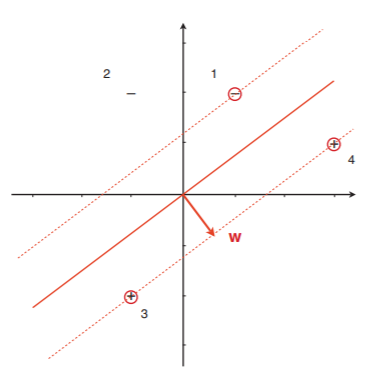
\includegraphics[width=0.5\linewidth]{images/svm.png}
	\caption{Przykład optymalnej linii maksymalizującej margines. Przypadki zaznaczone czerwonymi okręgami są wektorami wsparcia, źródło:~\cite{flach_2012} }
	\label{fig:svm}
\end{figure}

\section{Narzędzia do budowy gier}
Tworzenie gier komputerowych jest złożonym procesem, wymagającym pracy w~ramach wielu dziedzin naukowych. W~przypadku przygotowywania wysokobudżetowych produkcji przy pracy nad nimi potrafi pracować nawet kilkaset osób. Od projektantów poziomów, przez osoby zajmujące się przygotowaniem sceny fabularnej, grafików, kompozytorów muzyki aż po twórców oprogramowania, którzy łączą wcześniej przygotowane elementy w~jedną całość. To właśnie ci ostatni odpowiadają za ostateczną wersję gry, jej wygląd oraz optymalizację. 

Programiści tworzący końcową wersję gry, podczas tworzenia oprogramowania odpowiadającego za poszczególne jej elementy, muszą wziąć pod uwagę to, z~jakim rodzajem gry mają do czynienia. Każdy z~gatunków charakteryzuje się konkretnymi wymaganiami, które programista musi jak najlepiej odwzorować w~przygotowywanym kodzie gry. Dla przykładu gra wojenna powinna charakteryzować się balistyką pocisków oprogramowaną za pomocą wzorów fizycznych, realistycznym biegiem bohatera posiadającego określony poziom wytrzymałości, czy chociażby skutkami wybuchu granatu przedstawionymi jako uruchomione w~odpowiednim momencie elementy dźwiękowe i~graficzne. W~ostatnich latach dużą popularnością cieszą się gry z~gatunku Battle Royale~\cite{network_traffic_moll}, w~których kilkudziesięciu graczy ściera się ze sobą w~rozgrywce wieloosobowej. W~przypadku takich gier programiści muszą zwracać uwagę nie tylko na elementy związane z~rozgrywką, ale także na jak najdokładniejszą synchronizację klientów gry z~serwerem.

Ilość oraz złożoność elementów, które muszą zostać uwzględnione w~kodzie gry, powoduje, że stworzenie jej wyłącznie przy pomocy języków programowania jest niemal niemożliwe. Właśnie w~takim celu powstają oprogramowania nazywane silnikami do tworzenia gier. Umożliwiają one obsługę sterowania, grafiki, animacji, interakcji między obiektami, a~nawet sztucznej inteligencji, która może być jednym z~elementów gry. Silniki zwykle są dostępne w~formie środowisk programistycznych wprowadzających ułatwienia do zarządzania wcześniej wymienionymi elementami, jednocześnie przy tym nie rezygnując z~możliwości języków programowania. 

Istnieje mnóstwo narzędzi do tworzenia gier, jednak większość z~nich stanowią rozwiązania wykorzystywane jedynie w~obrębie danej firmy, która na potrzeby gry lub całej serii stworzyła silnik spełniający wymagania i~usprawniający proces tworzenia gier produkowanych przez daną spółkę. Przykładem może być rozwijany od lat IW engine, przy pomocy którego powstała seria gier Call of Duty. Z~tego właśnie powodu większość publikacji naukowych na temat gier komputerowych oparta jest o~darmowe silniki do gier. Kilka z~takich rozwiązań omówiono poniżej, zwracając uwagę na popularność, funkcje dostępne w~danym środowisku, języki, w~których można tworzyć aplikacje oraz na jakie platformy można wydać gry stworzone przy pomocy danego silnika.

\subsection{Godot}
Godot~\cite{godot_documentation} jest narzędziem umożliwiającym tworzenie gier na platformy takie jak Windows, macOS czy Linux, a~także na środowiska mobilne oraz webowe. Dużą zaletą Godota jest mały rozmiar edytora oraz dostępność na większość popularnych systemów operacyjnych. Skrypty oprogramowujące mechaniki gry mogą być tworzone przy pomocy języków C\#, C++, oraz wysokopoziomowego języka GDScript przygotowanego specjalnie dla tej platformy. Alternatywnym rozwiązaniem do tworzenia logiki gry są także skrypty wizualne (ang. \textit{visual scripting}) polegające na budowaniu kodu przy pomocy gotowych bloków, które będą zrozumiałe nie tylko dla programistów, ale również dla grafików czy animatorów. Dużym plusem, szczególnie dla osób, które dopiero zaczynają pracę z~Godotem, jest liczba przykładowych projektów, nie tylko w~formie gotowych gier, ale również pojedynczych elementów, takich jak sposoby padania światła czy to, w~jaki sposób stworzyć realistyczną wodę w~grze. 

\begin{figure}[h]
	\centering
	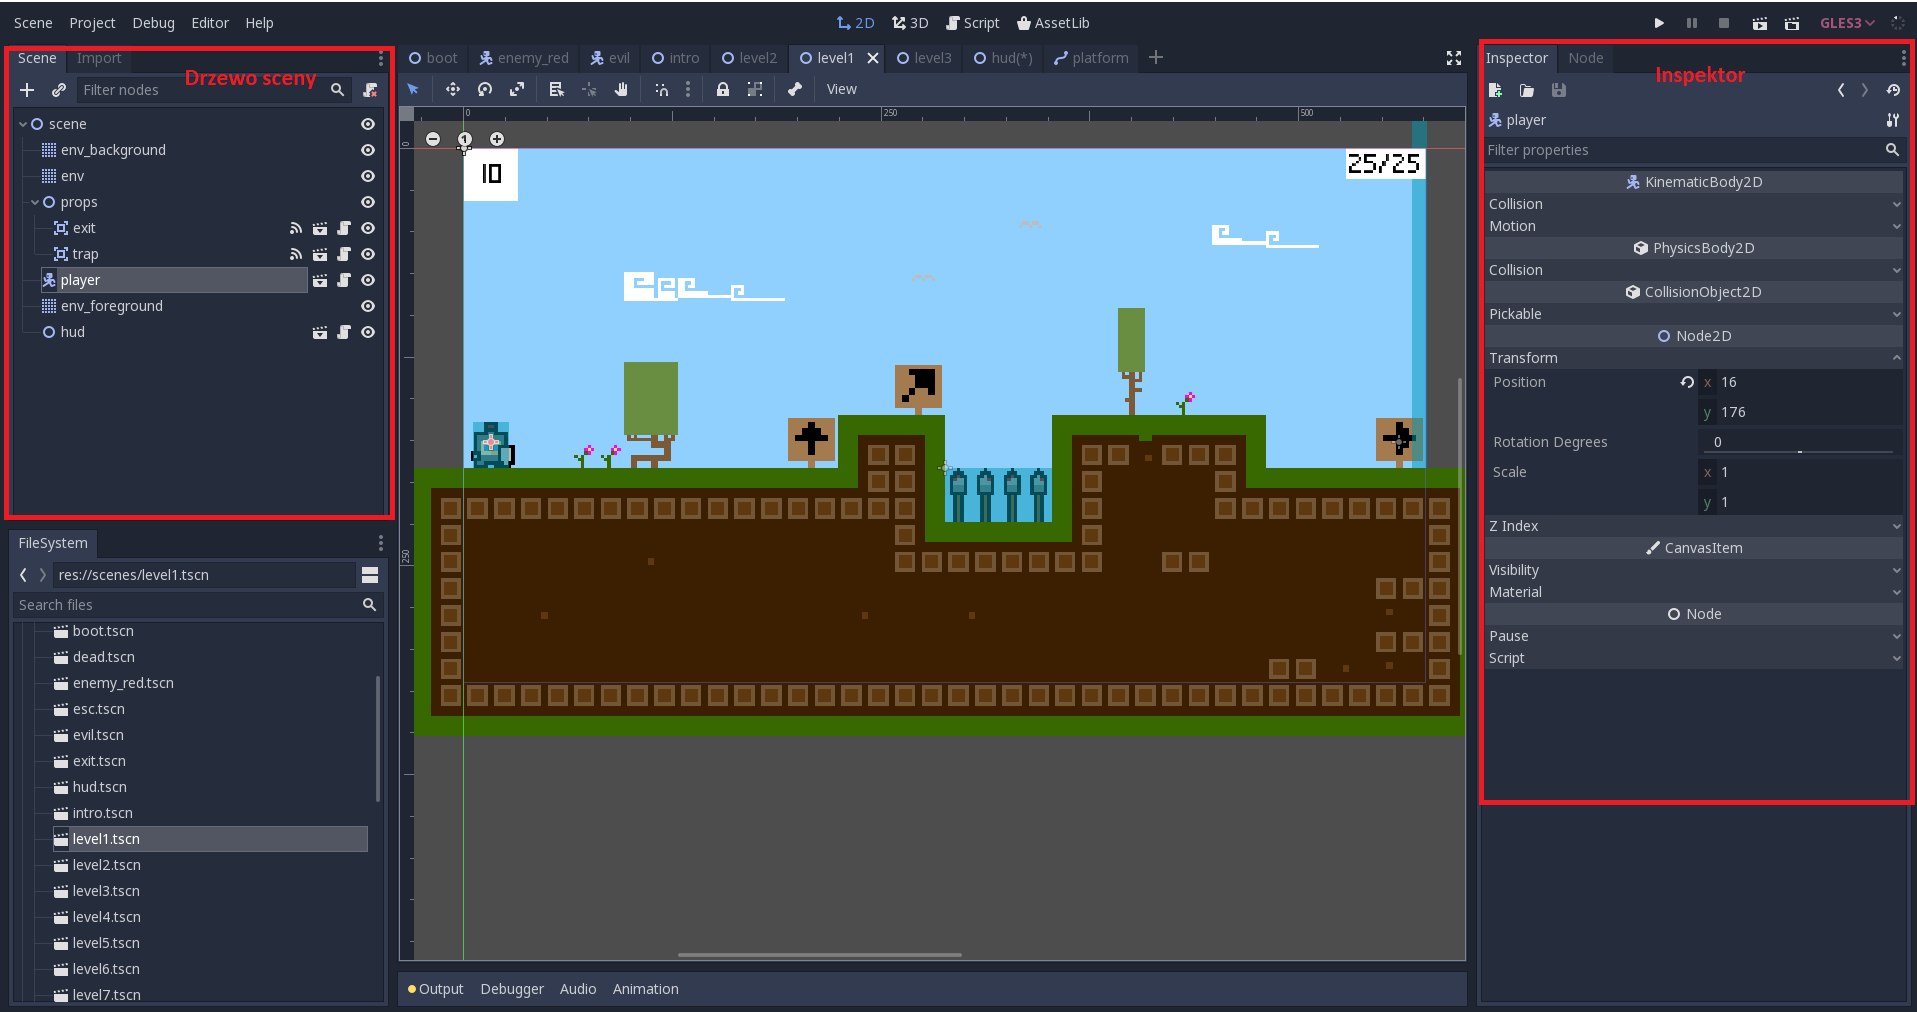
\includegraphics[width=0.9\linewidth]{images/godot_interface.png}
	\caption{Interfejs silnika Godot, po lewej stronie widać drzewo aktualnej sceny, źródło: opracowanie własne na podstawie~\cite{godot_documentation}}
	\label{fig:godot_interface}
\end{figure}

Projektowanie gier przy pomocy silnika Godot opiera się na budowaniu poszczególnych obiektów nazywanych scenami, które mogą następnie być łączone ze sobą na kolejnych scenach. Dzięki temu kolejne poziomy, a~nawet cały projekt mogą ostatecznie być opisane w~formie grafu powiązań. Takie rozwiązanie powoduje, że projekty przygotowane przy pomocy Godota są proste w~utrzymaniu podczas wspólnej pracy wielu osób. Każdy programista może w~danej chwili zająć się oddzielną sceną, nie powodując konfliktów z~elementami przygotowanymi przez inne osoby.

\subsection{Unity}
Unity jest silnikiem umożliwiającym tworzenie gier na o~wiele większą liczbę platform niż Godot~\cite{unity_manual}. Poza opisanymi wcześniej Windowsem, Linuxem, macOS'em oraz platformami mobilnymi i~webowymi, przy pomocy Unity można tworzyć gry na konsole współczesnej generacji oraz okulary wirtualnej i~rozszerzonej rzeczywistości. Sama platforma jest dostępna na systemy Windows oraz Mac, a~od niedawna twórcy starają się dostosować ją także na dystrybucje oparte o~jądro Linux. 

Projektowanie gier w~środowisku Unity polega na tworzeniu obiektów, do których przypisane są konkretne właściwości w~zależności od rodzaju stworzonego obiektu. Do każdego z~takich elementów mogą również zostać przyporządkowane skrypty odpowiadające za logikę działania obiektu, które tworzone są przy pomocy języka C\#. W~momencie tworzenia niniejszej pracy twórcy zapowiedzieli także dodanie skryptów wizualnych, co stanowi alternatywę dla osób niezaznajomionych z~programowaniem lub też z~samym językiem. Przygotowane elementy są umieszczane w~środowisku gry nazywanym sceną. Interfejs Unity pozwala na bardzo proste manewrowanie pomiędzy obiektami znajdującymi się na scenie, zarządzenie ich parametrami oraz powiązaniami między nimi.

\begin{figure}[h]
	\centering
	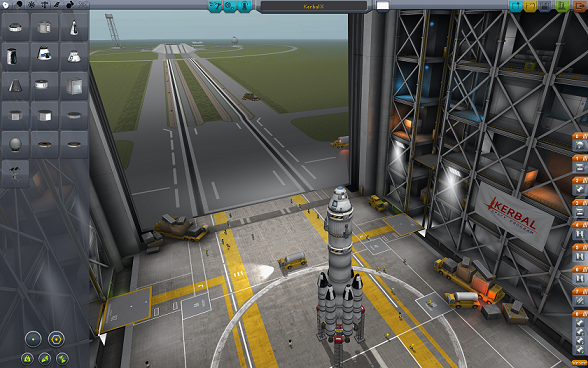
\includegraphics[width=0.7\linewidth]{images/kerbal_space_program.png}
	\caption{Kerbal Space Program, jedna z~najpopularniejszych gier stworzonych przy pomocy silnika Unity, źródło:~\cite{kerbal_your_enthusiasm}}
	\label{fig:kerbal_space_program}
\end{figure}

Unity jest obecnie jedną z~najpopularniejszych platform do tworzenia gier komputerowych. Przy jego pomocy powstało wiele znanych na świecie produkcji takich jak gry karciane Hearthstone i~Gwint, a~także gra symulacyjna Kerbal Space Program (rys. \ref{fig:kerbal_space_program}). Popularność ta przejawia się przede wszystkim w~postaci ogromnej liczby poradników dostępnych w~sieci, a~także aktywnej społeczności, która stale komunikuje się między sobą w~celu rozwiązania problemów występujących podczas tworzenia gier komputerowych. Dzięki temu, poza standardową dokumentacją, która także jest mocno rozbudowana, użytkownik ma dostęp do dodatkowych informacji uzyskanych od bardziej doświadczonych programistów. Cechą platformy, która mogła wpłynąć na jej popularność, jest także specjalnie przygotowany sklep zawierający zarówno płatne, jak i~darmowe dodatki rozszerzające możliwości silnika lub po prostu ułatwiające pracę przy konkretnym gatunku gry.

\subsection{Unreal Engine}
Unreal Engine jest narzędziem, które przez wiele lat było wykorzystywane jedynie do tworzenia dużych, komercyjnych gier. Do momentu wydania wersji trzeciej, projektowanie gier przy jego pomocy było ograniczone odpłatną licencją~\cite{unreal_manual}. Dopiero w~roku 2009~twórcy wydali oprogramowanie Unreal Development Kit, będące darmową wersją trzeciej wersji silnika, z~uszczuploną bazą gotowych modeli oraz bez dostępu do kodu źródłowego~\cite{udk_manual}. Dopiero kilka lat po wydaniu Unreal Engine 4~twórcy zdecydowali się na udostępnienie pełnej wersji oprogramowania za darmo. 

Spośród opisywanych rozwiązań, Unreal Engine jest najbardziej rozbudowanym. Podobnie do Unity umożliwia tworzenie gier na większość dostępnych platform, w~tym także okularów wirtualnej rzeczywistości. Językiem programowania wykorzystywanym do projektowania gier w~tym silniku jest C++, co można traktować jako wadę, ponieważ jest to język trudny i~wymagający dużo czasu na opanowanie. Z~drugiej strony jednak gry napisane przy pomocy C++ potrafią działać szybciej i~płynniej od rozwiązań stworzonych przy pomocy języków wysokopoziomowych. Ogromną zaletą silnika, która wyróżnia go na tle innych rozwiązań, jest dostęp do kodu źródłowego. Dzięki temu, twórcy gier mogą dostosować, a~nawet rozszerzyć możliwości platformy. 

\begin{figure}
	\centering
	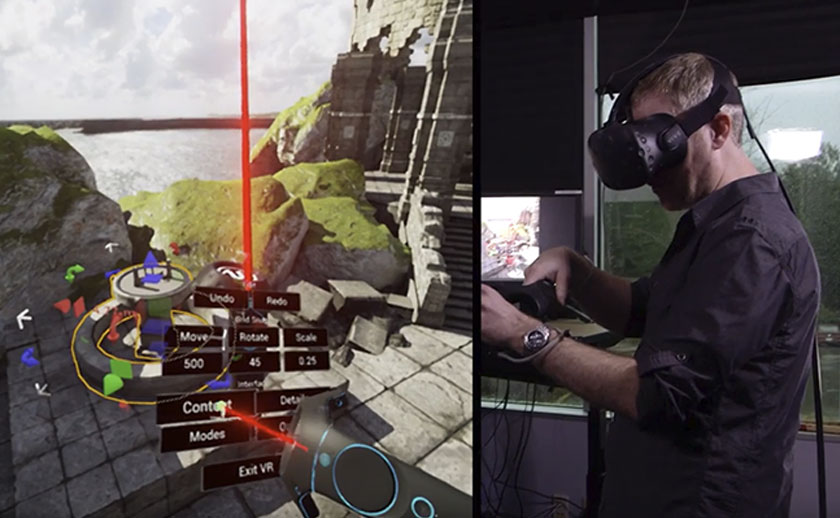
\includegraphics[width=0.7\linewidth]{images/unreal_vr_editor.jpg}
	\caption{Interfejs edytora Unreal Engine w~wirtualnej rzeczywistości, źródło:~\cite{unreal_manual}}
	\label{fig:unreal_vr_editor}
\end{figure}

Dla osób niepracujących z~kodem Unreal Engine udostępnia rozbudowany interfejs, pozwalający na stworzenie gry bez konieczności pisania kodu. Podobnie jak w~przypadku Unity, projekt gry składa się z~powiązanych ze sobą scen, tutaj nazywanych poziomami. Na każdej ze scen umieszczone są obiekty, nazywane aktorami, pomiędzy którymi zaprogramowane są interakcje specyficzne dla danej sceny. Osoba tworząca grę może zaprogramować jej logikę przy pomocy skryptów wizualnych. Tutaj warto opisać kolejny atut wyróżniający ten silnik na tle innych, którym jest możliwość korzystania z~edytora przy pomocy okularów wirtualnej rzeczywistości podczas tworzenia gier na tę platformę (rys. \ref{fig:unreal_vr_editor}). Twórca dostaje możliwość dokładnego zaprojektowania świata gry, patrząc na nią od razu z~perspektywy gracza. 

Unreal Engine jest obecnie drugą, tuż po Unity, najpopularniejszą otwartą platformą do gier. Przewaga Unity wynika tutaj nie z~większych możliwości silnika, ale z~jego otwartości od początku istnienia. Ponieważ jednak przez wiele lat Unreal Engine był wykorzystywany głównie w~rozwiązaniach komercyjnych, posiada rozbudowaną, złożoną dokumentację, która opisuje każdy fragment możliwości edytora. Po udostępnieniu darmowej wersji oprogramowania pojawiła się także duża ilość materiałów na temat tworzenia gier przy pomocy Unreal Engine, a~także urosła społeczność twórców gier, którzy wykorzystują ten silnik i~wymieniają się między sobą cennymi informacjami. 

\chapter{Architektura}
\label{cha:architektura}
Na podstawie analizy możliwych rozwiązań sprzętowych w~rozdziale~\ref{cha:specyfikacja} oraz przedstawionych poniżej założeń architektury platformy dokonano wyboru urządzeń, które będą stanowiły część sprzętową tworzonego interfejsu. W~tym rozdziale przedstawiono ich specyfikacje oraz argumenty, które przemawiają za wyborem każdego z~nich. Opisano także sposób montażu sprzętu.

\section{Założenia architektury sprzętowej}
Aby wybrać odpowiedni dla przygotowywanego prototypu interfejsu zestaw urządzeń, określone zostały założenia i~wymagania, jakie powinny one spełniać:
\begin{enumerate}
	\item Platforma sprzętowa powinna być lekka, aby używanie jej przez gracza nie powodowało dyskomfortu, który może wpłynąć negatywnie na jakość odbieranych danych.
	\item Dokładność dostępnych sensorów powinna być jak największa, aby mieć pewność odczytywanych zachowań użytkownika.
	\item Urządzenie powinno być łatwe w~obsłudze, zarówno w~kwestii jego zamontowania, jak i~uruchomienia odczytów. Jednocześnie powinno charakteryzować się jak najmniejszą inwazyjnością podczas pomiaru, aby zminimalizować dyskomfort użytkownika.
	\item Dla wybranego sprzętu powinno być dostępne oprogramowanie umożliwiające odczyt sygnałów w~wybranym środowisku do tworzenia gier. Najlepiej, gdyby rozwiązanie było dostępne w~postaci biblioteki oferowanej przez twórcę narzędzia lub rozszerzenia silnika, które umożliwi odbieranie danych.
	\item Urządzenie powinno mieć możliwość połączenia bezprzewodowego, najlepiej przy pomocy technologii Bluetooth lub innego protokołu umożliwiającego bezprzewodowy przesył danych.
	\item Przynajmniej jedno z~urządzeń powinno umożliwiać odczyt pracy serca w~postaci pulsu lub sygnału z~elektrokardiogramu. Pomiar tętna jest jedną z~podstawowych metod umożliwiających określenie zmian w~stanie emocjonalnym użytkownika.
	\item Przynajmniej jedno z~urządzeń powinno umożliwiać odczytywanie ruchów mięśni. Uzyskane sygnały mogą być wykorzystane do wpływania na rozgrywkę w~zależności od aktywności mięśniowej użytkownika w~danej partii ciała.
\end{enumerate}


\section{Garmin HRM-Run}
Garmin HRM-Run jest jednym z~wielu dostępnych czujników tętna produkowanych przez firmę Garmin. Urządzenie zbudowane jest z~modułu zawierającego elektronikę odpowiedzialną za interpretację oraz wysyłanie odczytywanych danych. Zasilany jest on baterią CR2032 i~zamontowany jest na elastycznej opasce, umożliwiającej zamontowanie opaski na klatce piersiowej. Sama opaska zawiera dwie elektrody odpowiadające za odczyt sygnałów fizjologicznych, które następnie są przekazywane w~formie informacji na temat pracy serca. 

Czujnik, poza podstawowym pomiarem liczby uderzeń na minutę, pozwala na pozyskiwanie dodatkowych informacji na temat zmienności rytmu zatokowego w~postaci odstępów czasowych pomiędzy kolejnymi załamkami R, czyli szczytami kompleksów QRS. Na podstawie tej informacji można określić stan zdrowotny użytkownika lub zmiany jego stanu emocjonalnego. Dla przykładu nagłe spadki w~zmienności rytmu zatokowego mogą sygnalizować możliwość odczuwania stresu przez użytkownika. HRM-Run umożliwia także zbieranie danych na temat dynamiki biegu, takich jak liczba kroków na minutę, czas kontaktu z~podłożem czy długość kroku. Ze względu na charakter pracy, która skupia się głównie na tematyce gier komputerowych, pomiary te nie były brane pod uwagę. 

Urządzenie HRM-Run zostało wybrane, ponieważ stanowi pewien kompromis pomiędzy dokładnością odczytów a~rozmiarami i~wygodą użytkowania. W~porównaniu do inteligentnych opasek, charakteryzujących się najwyższym poziomem komfortu spośród omówionych w~rozdziale \ref{cha:specyfikacja} platform sprzętowych umożliwiających pomiar tętna, Garmin HRM-Run pozwala na o~wiele dokładniejsze odczyty, nie powodując przy tym dyskomfortu podczas użytkowania. Jest to możliwe dzięki wykorzystaniu elastycznej opaski ze wbudowanymi suchymi elektrodami, które, w~przeciwieństwie do fotopletyzmografu odpowiadającego za optyczny odczyt tętna w~inteligentnych opaskach, odbierają sygnały elektryczne bezpośrednio z~ciała użytkownika. Informacje te są następnie interpretowane do danych w~postaci wykrycia kolejnych uderzeń serca. Opaski natomiast charakteryzują się dużymi opóźnieniami w~stosunku do aktualnego tętna użytkownika, co w~przypadku rozpoznawania emocji w~sposób ciągły całkowicie eliminuje je jako akceptowalne rozwiązanie. Jednocześnie elastyczna opaska, do której przymocowany jest moduł, w~bardzo prosty sposób jest zakładana przez użytkownika na klatce piersiowej. Takie umiejscowienie i~brak kabli łączących elektrody z~głównym modułem sprawia, że użytkownik nie czuje dyskomfortu podczas noszenia urządzenia. W~podobny sposób Garmin HRM-Run można porównać z~omawianym wcześniej BITalino (r)evolution kit. W~tym przypadku można zauważyć sytuację odwrotną niż przy porównaniu z~inteligentnymi opaskami. BITalino oferuje bardzo dokładny pomiar pracy serca, nie tylko w~formie liczby uderzeń na minutę, ale także pełnego elektrokardiogramu umożliwiającego o~wiele szerszą analizę pracy serca. Niestety, odczyt wymaga zamocowania przyklejanych elektrod, które połączone są przewodami z~sensorem, a~następnie z~samym BITalino. Taki sposób montażu może wpłynąć negatywnie na komfort podczas gry, co nie wystąpi w~przypadku urządzenia HRM-Run.

Innym aspektem decydującym o~wyborze tej platformy sprzętowej, jest obsługa dwóch protokołów bezprzewodowego przesyłania danych. Poza standardowym połączeniem dzięki technologii Bluetooth HRM-Run wykorzystuje także protokół ANT+ rozwijany przez firmę Garmin. Jego główną zaletą jest brak ograniczeń co do ilości urządzeń mogących odbierać dane z~czujnika. W~przeciwieństwie do technologii Bluetooth, która ogranicza połączenie do jednego lub w~przypadku Bluetooth Smart, dwóch urządzeń, pomiar przy pomocy protokołu ANT+ umożliwia jednoczesne odczytywanie danych w~grze i~monitorowanie pracy serca przy pomocy innych narzędzi korzystających z~tego protokołu. Twórcy ANT+ udostępniają szeroką dokumentację oraz biblioteki umożliwiające odczyt w~wielu językach programowania, od C++, C\#, aż po dedykowane implementacje dla systemu Android.

\begin{figure}
	\centering
	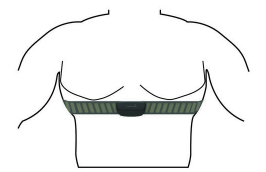
\includegraphics[width=0.5\linewidth]{images/garmin_hrm_placement.png}
	\caption{Miejsce montażu czujnika tętna Garmin HRM-Run, źródło:~\cite{garmin_manual}}
	\label{fig:garmin_placement}
\end{figure}

\section{BITalino (r)evolution kit}
BITalino (r)evolution Plugged Kit BT jest urządzeniem produkowanym przez firmę PLUX Wireless Biosignals przeznaczonym do tworzenia platform, w~których zawarte są elementy wymagające informacji na temat sygnałów fizjologicznych. Główny element narzędzia stanowi płytka zbudowana z~następujących części~\cite{bitalino_documentation}:
\begin{itemize}
	\item 10~złącz UC-E6, w~ramach których można wyróżnić: 6~wejść analogowych, 1~wejście cyfrowe, 1~wyjście cyfrowe, 1~złącze mogące pracować w~trybie wejścia lub wyjścia cyfrowego oraz 1~złącze PWM, do którego może zostać podłączony przetwornik DAC lub dioda LED. Złącza są podzielone na 2~grupy w~oddzielnych segmentach.
	\item Mikrokontroler z~mikroprocesorem oraz stykami umożliwiającymi połączenie każdego z~segmentów w~sposób inny niż standardowy
	\item Segment zasilający, zawierający włącznik, gniazdo ładownia w~formie złącza micro-USB oraz złącze JST, do którego podłączana jest bateria 3.7V zasilająca całą płytkę.
	\item Moduł Bluetooth odpowiadający za przesył danych z~płytki.
\end{itemize}

W ramach przygotowywanego interfejsu, z~dostępnych sensorów opisanych w~rozdziale \ref{cha:specyfikacja} wybrany został jedynie moduł zawierający elektromiogram mierzący napięcie mięśni podskórnych. Głównym powodem takiego wyboru są dwie główne wady urządzenia dotyczące komfortu użytkowania. Są to przewody łączące płytkę z~sensorem oraz elektrody mocowane z~drugiej strony przewodów. Choć z~perspektywy eksperymentów naukowych użycie elektrod żelowych przyklejanych do skóry nie jest problemem, to w~przypadku środowiska gier komputerowych standardowy użytkownik może odczuwać dyskomfort lub w~ogóle zrezygnować z~używania urządzenia ze względu na jego inwazyjność.

Głównym powodem wyboru BITalino oraz samego modułu EMG jest wykorzystanie sygnałów fizjologicznych do kontrolowania gry w~świadomy sposób. Odczyt zmian napięcia mięśni podskórnych może pozwolić na wykrycie, kiedy i~jak mocno są one używane, co może następnie zostać wykorzystane do zaimplementowania mechanik w~grze uruchamianych na podstawie konkretnych reakcji mięśniowych. Kolejnym powodem wykorzystania platformy sprzętowej jest możliwość sprawdzenia, w~jakim stopniu użytkownik tak naprawdę odczuwa dyskomfort podczas używania elektrod przyklejanych do skóry. Pozwoli to stwierdzić, czy urządzenia takie jak BITalino, które umożliwiają wykonanie dokładnych pomiarów dzięki wykorzystaniu elementów bliższych rozwiązaniom medycznym, mogłyby przyjąć się jako stały element stanowiska do gier.

Ponieważ odczyty z~elektromiogramu mają posłużyć jako pewien element kontroli nad grą, jako miejsce, do którego podłączone będą elektrody, wybrano przedramię, ponieważ ruch mięśni znajdujących się w~tamtej części ciała może być precyzyjny. Dzięki temu użytkownik w~prosty sposób, poprzez ruchy nadgarstka lub dłoni, może kontrolować napięcie mięśni w~trakcie rozgrywki. Sposób montażu elektrod został przedstawiony na rysunku~\ref{fig:bitalino_placement}. Elektrody czerwona i~czarna powinny znajdować się na wewnętrznej części przedramienia, równolegle do niego, stosunkowo blisko siebie. Elektroda referencyjna, w~BITalino oznaczona kolorem białym, powinna znajdować się na wystającej kości łokciowej.
\begin{figure}
	\centering
	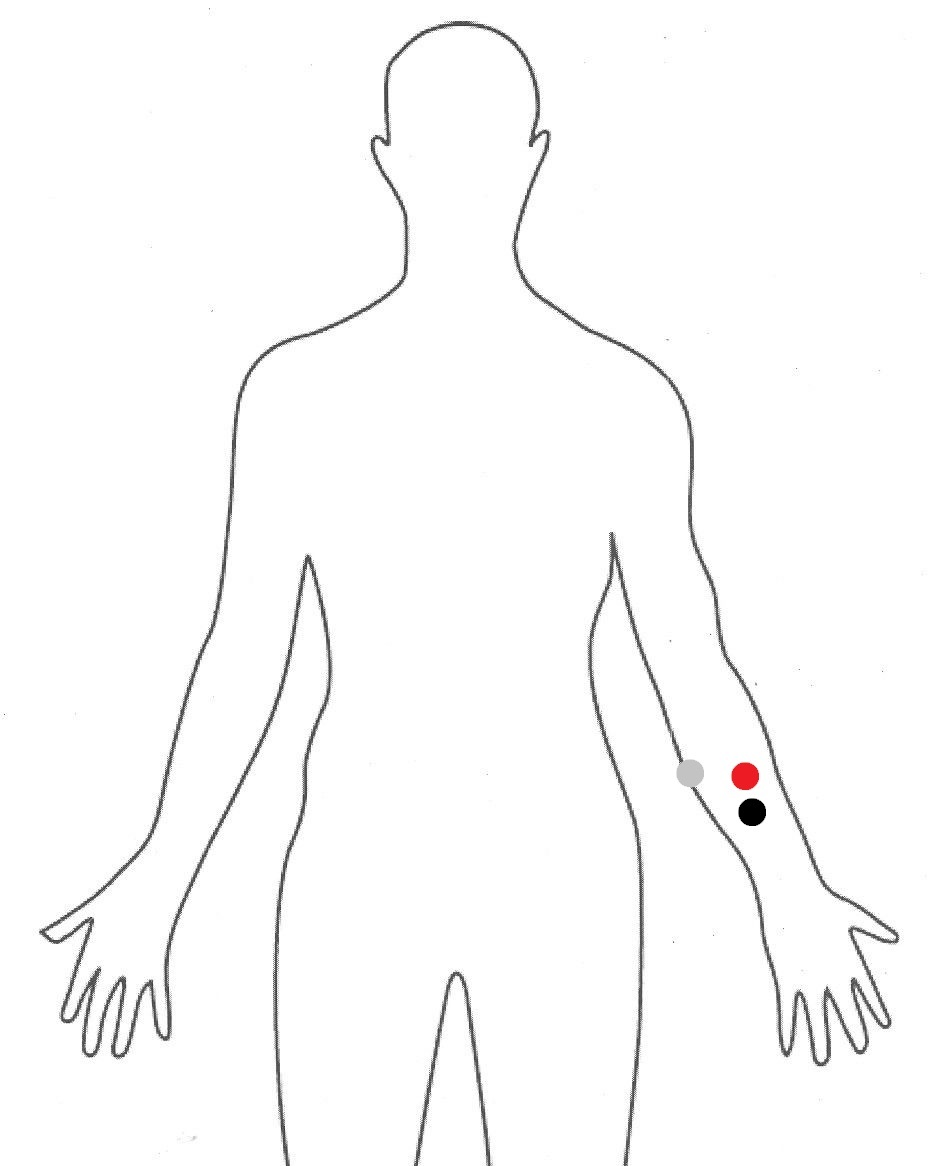
\includegraphics[height=0.3\textheight]{images/bitalino_placement.jpg}
	\caption{Sposób przypięcia elektrod dla sensora EMG,  kolor czerwony oznacza elektrodę dodatnią, czarny ujemną, a~szary elektrodę referencyjną}
	\label{fig:bitalino_placement}
\end{figure}

\section{DualShock 4}
DualShock 4~jest urządzeniem produkowanym przez firmę Sony, stworzonym początkowo jako kontroler do konsoli PlayStation 4. Na przyciski dostępne na jego powierzchni składają się~\cite{dualshock_specification}:
\begin{itemize}
	\item 2~gałki analogowe, gdzie dla każdej z~nich odczyty interpretowane są jako ciągły sygnał wejściowy przedstawiony w~dwóch wymiarach.
	\item Pad kierunkowy (ang. \textit{d-pad}) stanowiący cyfrowy odpowiednik gałki analogowej. Lewy i~prawy przycisk odpowiadają wartościom granicznym osi horyzontalnej, górny i~dolny są przypisane w~podobny sposób do osi wertykalnej.
	\item 9~przycisków cyfrowych, na które składają się: 4~przyciski akcji (trójkąt, kwadrat, krzyżyk, kółko), L3 i~R3 zamontowane pod gałkami analogowymi oraz przyciski PS, SHARE i~OPTIONS, domyślnie służące do zarządzania opcjami konsoli.
	\item 2~przyciski L1 i~R1, dla których wykrycie wciśnięcia opiera się na sile nacisku na przycisk.
	\item 2~analogowe spusty L2 i~R2, których wciśnięcie jest odczytywane jako sygnał w~określonym zakresie wartości.
	\item Dwupunktowy panel dotykowy, posiadający także możliwość kliknięcia go.
\end{itemize}
Innymi elementami widocznymi na urządzeniu są wbudowany głośnik, wejście słuchawkowe Jack 3.5mm, umieszczony na froncie pasek świetlny RGB oraz złącze micro-USB służące do ładowania i~podłączenia kontrolera w~przypadku braku połączenia Bluetooth. Kontroler, wraz ze wszystkimi opisanymi powyżej elementami, został przedstawiony na rysunku~\ref{fig:hardware}.

Poza widocznymi elementami Dualshock 4~posiada także wbudowane moduły wibrujące, żyroskop oraz akcelerometr. To właśnie dwa ostatnie z~wymienionych elementów wpłynęły na wybór urządzenia jako części przygotowywanego interfejsu. W~porównaniu do innych dostępnych kontrolerów, poza klasycznym wykorzystaniem narzędzia jako sposobu kierowania postacią w~grze, akcelerometr wbudowany w~DualShocka może posłużyć jako źródło danych, które w~pośredni sposób mogą określać pewne elementy stanu emocjonalnego użytkownika. Bardziej pobudzony gracz, może zupełnie nieświadomie poruszać kontrolerem, natomiast brak zmian w~odczytach może sugerować, że użytkownik jest skupiony lub znudzony. W~porównaniu do określania ilości kliknięć na myszy i~klawiaturze w~danym czasie, wykorzystanie akcelerometru jest lepszym rozwiązaniem, ponieważ ruchy dłoni gracza trzymającego kontroler są instynktowne w~sytuacjach wywołujących pobudzenie. Sceny wywołujące nagły strach, mogą doprowadzić do ruchu całego ciała, natomiast sytuacje powodujące uczucie złości lub desperacji mogą wywołać subtelne przesunięcie pozycji rąk na kontrolerze, co wywoła zmianę wartości na akcelerometrze. Interpretacja tych danych oraz odczytów pracy serca pozwoli na dokładniejsze określenie, jaką emocję odczuwa gracz w~danym momencie.

Problemem, który warto zaznaczyć w~przypadku DualShocka, jest ograniczenie dostępności oprogramowania pozwalającego odczytywać pomiary z~akcelerometru. Z~powodu licencji narzuconych przez producenta, większość dodatków i~bibliotek wykorzystywanych w~silnikach do gier jest dostępnych wyłączenie w~wersji płatnej, a~oficjalne oprogramowanie od twórców jest udostępniane wyłącznie osobom zatwierdzonym przez Sony jako projektanci gier na konsolę PlayStation 4. Jednakże, pomimo wspomnianego ograniczenia, zdecydowano się na wybór Dualshocka 4~jako części przygotowywanego interfejsu.

\begin{figure}
	\centering
	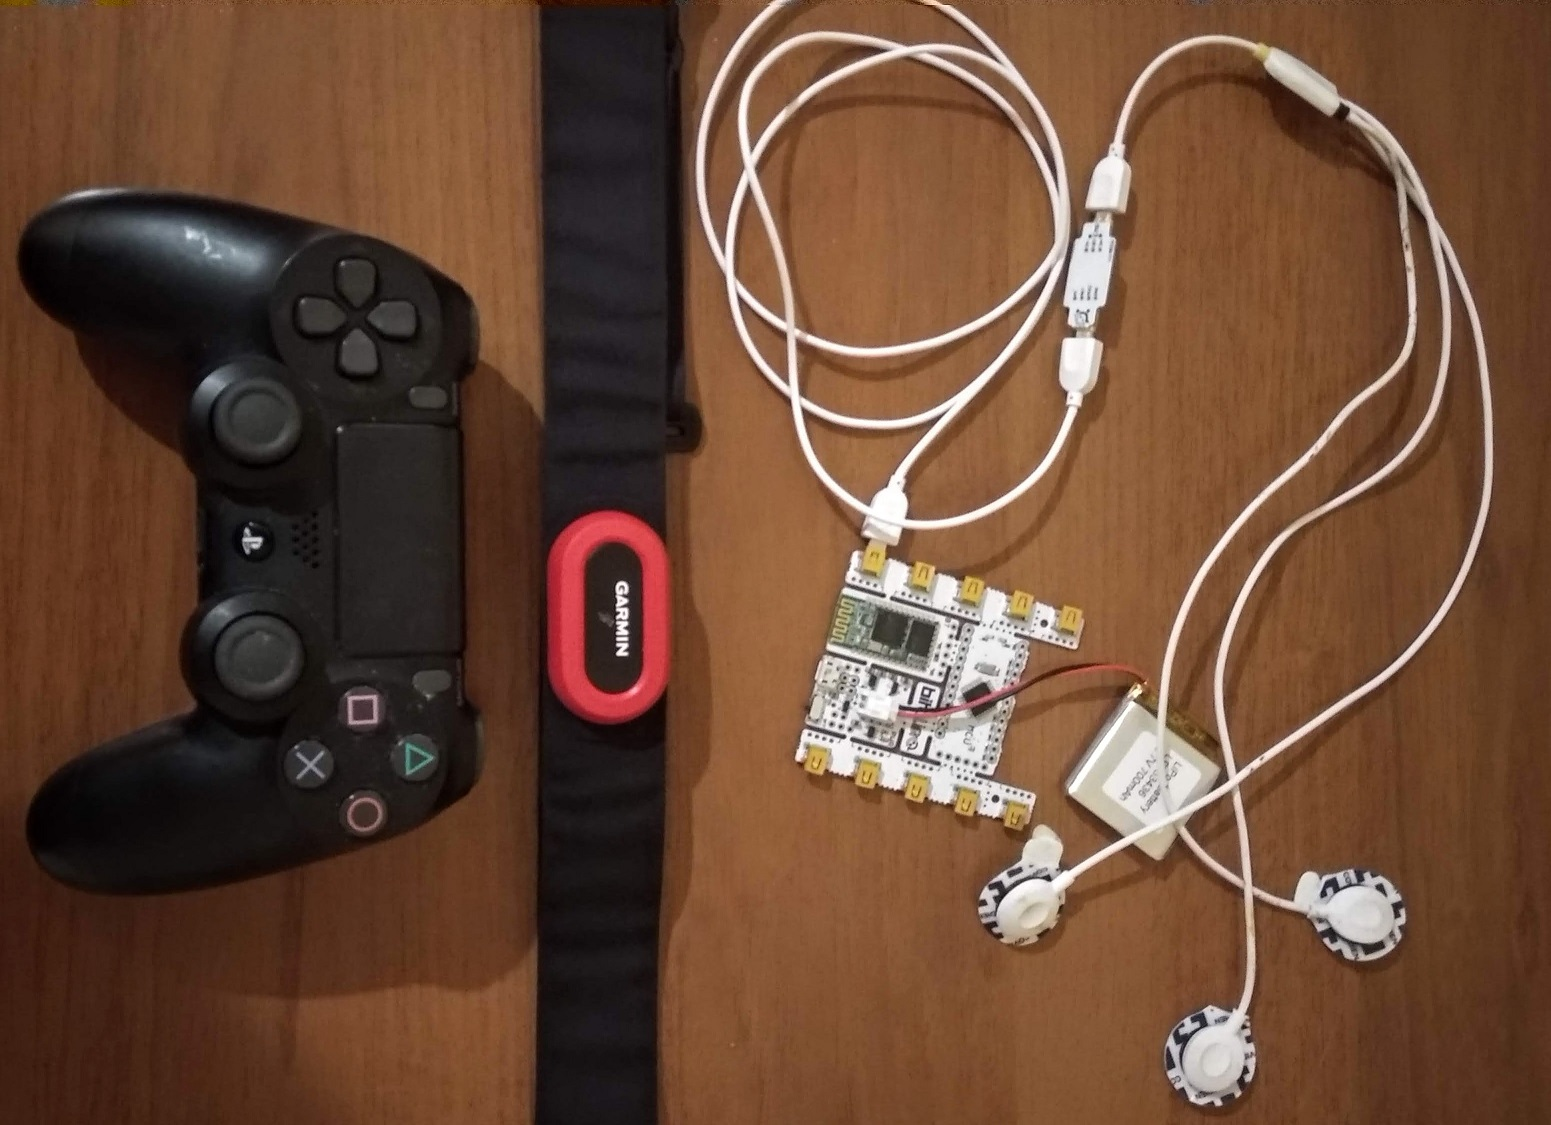
\includegraphics[width=0.7\linewidth]{images/hardware.jpg}
	\caption{Moduły sprzętowe wykorzystywane w~platformie. Od lewej: kontroler DualShock 4, czujnik tętna Garmin HRM-Run, BITalino z~modułem EMG}
	\label{fig:hardware}
\end{figure}

Na rysunku~\ref{fig:hardware} przedstawiony został pełen zestaw urządzeń wykorzystanych w~przygotowywanym interfejsie. Pozyskane z~nich pomiary zostaną wykorzystane do rozpoznania stanu emocjonalnego gracza, a~także do kontrolowania mechanik wykorzystywanych w~grze. Dokładny opis sposoby odczytu danych oraz jak będzie wyglądał model do predykcji emocji użytkownika, zostaną opisane w~rozdziałach~\ref{cha:predykcja} i~\ref{cha:implementacja}.
\chapter{Mechanizm predykcji emocji}
\label{cha:predykcja}
\section{Rozpoznawanie emocji}
\subsection{Dane uczące}
Jakie datasety, krótki opis
\subsection{Przetworzenie danych}
Opis preprocessingu, wykorzystane cechy
\subsection{Wybór modelu}
Ewaluacja w hyperopt, statystyki skuteczności, ostateczny wybór modelu
\chapter{Implementacja}
\label{cha:implementacja}
W ramach niniejszej pracy magisterskiej stworzono grę elektroniczną, w~której miał zostać wykorzystany przygotowywany prototyp interfejsu do  odczytu zmianów stanów emocjonalnych i~zachowań gracza. Na podstawie analizy silników do tworzenia gier przeprowadzonej w~rozdziale~\ref{cha:specyfikacja} zdecydowano się na wykorzystanie silnika Unity. Głównym powodem takiej decyzji była przede wszystkim ilość materiałów o~tematyce tworzenia gier przy pomocy właśnie silnika Unity, a~także dostępność rozwiązań, które pozwalały na prostą komunikację z~urządzeniami opisanymi w~rozdziale~\ref{cha:architektura}. 

\section{Podstawowe założenia}
Zanim rozpoczęto implementację gry, zostały określone założenia i~wymagania implementacyjne i~projektowe, według których następnie została zbudowana gra:
\begin{enumerate}
	\item Gra powinna zawierać mechaniki afektywne, które modyfikują rozgrywkę w~zależności od zachowania lub stanu emocjonalnego gracza.
	\item Jednym z~elementów implementacyjnych powinien być moduł umożliwiający komunikację z~urządzeniami opisanymi w~rozdziale~\ref{cha:architektura}. Moduł powinien także komunikować się z~serwerem zawierającym moduł do predykcji emocji oraz w~sposób prosty udostępniać zmiany stanu emocjonalnego użytkownika i~jego zachowań. 
	\item Gra powinna mieć możliwość wyboru jednego z~dwóch trybów gry: podstawowego, zawierający standardowe mechaniki gry, oraz wersję afektywną.
	\item Rozgrywka powinna być powtarzalna, tak aby w~trakcie przeprowadzania badań, każdy z~uczestników mógł doświadczyć tych samych elementów gry.
\end{enumerate}

\section{Implementacja gry}
%Opis gry, które elementy za co odpowiadają
Ponieważ przygotowywana gra miała być wykorzystana do przeprowadzenia eksperymentów w~celu ewaluacji opracowanego rozwiązania, zdecydowano, że będzie to gra jednoosobowa. W~trakcie rozgrywki gracz wciela się w~rolę kapitana statku kosmicznego, który musi walczyć z~przeciwnikami, aby przeżyć. Jego zadaniem jest sterowanie statkiem i~pokonanie jak największej liczby przeciwników przy pomocy dostępnego wyposażenia. Rozgrywka podzielona jest na poziomy, w~których trakcie gracz musi zdobyć określoną liczbę punktów. Na każdym z~poziomów dookoła statku generowanych jest kilka rodzajów wrogich statków, których schemat i~szybkość generowania są zróżnicowane w~zależności od poziomu. Z~każdym kolejnym poziomem pojawiają się nowe rodzaje jednostek, które mogą nie tylko wlatywać w~gracza lub do niego strzelać pojedynczymi pociskami, ale również wybuchać w~jego pobliżu, posiadać większą wytrzymałość lub strzelać innymi rodzajami pocisków. Każdy z~przeciwników ma także przypisaną ilość punktów, która jest dodawana do puli po zniszczeniu go. Aby przejść do kolejnego poziomu, gracz musi zebrać odpowiednią liczbę punktów.

Gracz posiada ograniczoną liczbę punktów życia, która zwiększa się po przejściu każdego z~poziomów. Aby urozmaicić rozgrywkę, dookoła gracza mogą pojawić się także wzmocnienia w~postaci innych broni oraz elementów leczących. Innym elementem mającym mocno wpłynąć na rozgrywkę jest moc specjalna, która umożliwia graczowi wypuszczenie fali w~kształcie okręgu, która natychmiastowo niszczy wrogie statki. Ponieważ umiejętność ta bardzo ułatwia rozgrywkę, gracz jest w~stanie użyć jej jedynie co określony czas. 

Aby wyrównać poziom gry i~nie znudzić gracz powtarzalną rozgrywką, każdy z~poziomów posiada także dodatkowy tryb, który jest trudniejszy niż podstawowa rozgrywka. Tryb ten jest uruchamiany na pewien określony czas po spełnieniu specjalnych warunków, które w~zależności od wersji gry są inne. W~trakcie trwania trybu trudnego schemat generowania przeciwników jest zmieniany na ich trudniejsze wersje, posiadające większą ilość życia i~inne umiejętności. Zmienia się także szybkość generowania przeciwników, która zostaje podwojona.

Cała gra została stworzona w~stylu dwuwymiarowym. Na rysunku~\ref{fig:ui} przedstawiony został fragment przykładowej rozgrywki. Oznaczone elementy interfejsu użytkownika to kolejno:
\begin{enumerate}
	\item \textbf{Pasek wskazujący poziom życia bohatera}. Warto zwrócić uwagę na brak oznaczenia dokładnej ilości punktów życia. Ukrycie tej informacji zmusza użytkownika do kontrolowania poziomu życia w~trakcie gry, a~także do unikania wszystkich przeciwników, niezależnie od tego, jakie obrażenia zadają.
	\item \textbf{Ikony aktualnie wybranej broni i~dostępności mocy specjalnej}. Służą one przede wszystkim jako elementy informacyjne. Wskazanie aktualnie wybranej broni pozwala graczowi między innymi na zorientowanie się, czy wzmocnienie w~postaci innego typu pocisków jest lepsze od aktualnie posiadanego. Ikona mocy specjalnej natomiast jest nie tylko wskazaniem jej dostępności. W~trakcie czasu odnowienia mocy specjalnej ikona ta spełnia funkcję orientacyjnego licznika, który wskazuje użytkownikowi, kiedy ponownie będzie mógł z~niej skorzystać.
	\item \textbf{Ilość punktów zdobytych przez gracza oraz pasek postępu dla danego poziomu}. Podobnie jak w~przypadku ilości punktów życia, pasek postępu wskazuje jedynie orientacyjny postęp gracza na danym poziomie, dzięki czemu użytkownik nie jest do końca pewien, kiedy ukończy poziom. Z~drugiej strony wyświetlana jest suma punktów zdobytych w~trakcie całej rozgrywki, co stanowi pewnego rodzaju motywację dla gracza, aby zdobyć jak najwyższy wynik.
\end{enumerate}

\begin{figure}
	\centering
	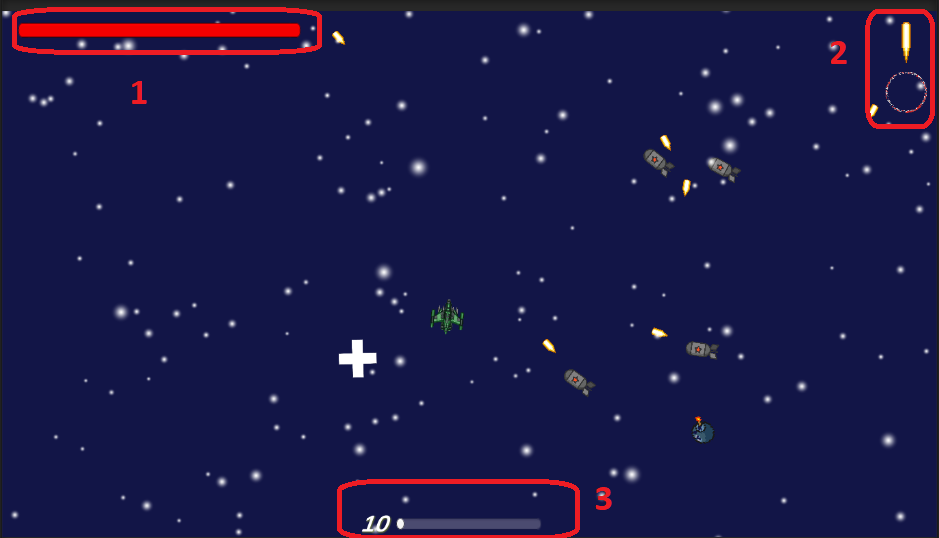
\includegraphics[width=0.7\linewidth]{images/ui.png}
	\caption{Ekran gry z~oznaczonymi elementami interfejsu użytkownika}
	\label{fig:ui}
\end{figure}

Tak jak zostało wspomniane na początku rozdziału, do implementacji gry wykorzystano silnik Unity. W~momencie tworzenia projektu gry zdecydowano się na użycie wersji 2018.3.0f2, która jest przeznaczona do tworzenia gier na systemy operacyjne oparte o~architekturę 64-bitową. Ponieważ projektowanie gier przy pomocy tego silnika jest oparte na tworzeniu obiektów, które są wprowadzane w~interakcje pomiędzy sobą, a~logika za to odpowiadająca zawarta jest w~skryptach dołączanych do obiektów, zdecydowano się na stworzenie hierarchii, w~której pierwszym poziomem są poszczególne elementy rozgrywki w~postaci obiektów tworzonych na scenie gry, drugim natomiast są skrypty odpowiadające za logikę danego obiektu lub innych elementów gry takich jak interfejs użytkownika czy postępy gracza. Do obiektów stanowiących główne elementy świata gry należą:
\begin{enumerate}
	\item \textbf{Player} reprezentujący statek, którym kieruje gracz. Poza elementami graficznymi zawiera on następujące skrypty związane ze sterowanym statkiem:
	\begin{itemize}
		\item \textbf{PlayerController}, opisujący sposób poruszania się kontrolowanego statku. Przy jego pomocy ustawiana są także szybkość poruszania się oraz czas potrzebny na wyhamowanie statku.
		\item \textbf{PlayerShooter}, odpowiadający za logikę strzelania przy pomocy wybranej broni, a~także za użycie mocy specjalnej. Jej głównym zadaniem jest zarządzanie tworzeniem pocisków i~aktywacji animacji oraz dźwięków związanych ze strzałem lub aktywacją mocy specjalnej. Skrypt odpowiada także za integrację z~elementami interfejsu użytkownika odpowiedzialnymi za wyświetlanie aktualnie używanej broni i~dostępności mocy specjalnej. Skrypt umożliwia także zmianę aktualnie używanej broni oraz zarządzanie parametrem czasu odnowienia mocy specjalnej. 
		\item \textbf{Player}, odpowiadający za kontrolowanie życia postaci. Mowa tutaj nie tylko o~zmniejszaniu życia po przyjęciu obrażeń lub zwiększaniu podczas leczenia bohatera, ale również ustawianiu nowej wartości maksymalnej ilości punktów życia po zakończeniu poziomu. Skrypt ten zarządza elementem interfejsu użytkownika odpowiedzialnym za wyświetlanie aktualnej ilości punktów życia. Kontroluje także wywołanie animacji i~dźwięków uruchamianych po śmierci bohatera, a~także oddelegowanie akcji odpowiedzialnych za zatrzymanie gry do obiektów sterujących rozgrywką.
	\end{itemize}

	\item \textbf{Obiekty reprezentujące przeciwników}. Każdy z~nich różnił się przypisanymi elementami graficznymi oraz skryptami, które mogą różnić się w~zależności od typu przeciwnika. Do skryptów sterujących logiką przeciwników należą:
	\begin{itemize}
		\item \textbf{Enemy}, odpowiadający przede wszystkim za zarządzanie poziomem życia przeciwnika, zmniejszaniu go po zadaniu obrażeń przez gracza, zmianie elementów graficznych w~zależności od ilości punktów życia przeciwnika, oraz za wywołanie animacji i~dźwięków mających nastąpić po śmierci przeciwnika. Skrypt posiada także parametr związany z~ilością obrażeń zadawanych podczas zderzenia z~graczem i~zarządza samą akcją kolizji, zabierając graczowi ustaloną ilość punktów życia.
		\item \textbf{EnemyMovement}, odpowiadający za sposób poruszania się przeciwnika. W~zależności od typu wroga, skrypt zarządza czy ma się on zbliżać do gracza, okrążać go, czy może stać w~miejscu. Zawiera on parametry dotyczące szybkości przeciwnika, maksymalnej odległości od gracza, oraz dystansu od niego, na jakim część przeciwników ma się zatrzymać.
		\item \textbf{EnemyShooter}, odpowiadający za kontrolę strzałów przeciwnika, ich szybkość, stworzenie pocisków oraz wywołanie efektów dźwiękowych strzału. Skrypt ten jest przypisywany wyłącznie do przeciwników typu strzelającego.
		\item \textbf{EnemyBomber}, zarządzający logiką wybuchu przeciwnika. Kontroluje przede wszystkim zadanie graczowi obrażeń i~odepchnięcie innych przeciwników, jeśli znajdują się w~zadanej przez parametr odległości. Odpowiada także za uruchomienie animacji oraz dźwięku związanych z~odliczaniem do wybuchu.
	\end{itemize}
	
	\item \textbf{Obiekty reprezentujące wzmocnienia, które gracz może zdobyć w~trakcie rozgrywki}. Poza elementami graficznymi, w~zależności od rodzaju wzmocnienia, każdy z~nich ma przypisany do siebie następujące skrypty:
	\begin{itemize}
		\item \textbf{PowerUp}, odpowiadający za wywołanie efektu wzmacniającego gracza, oraz ciągły obrót obiektu wzmocnienia. Jest to skrypt abstrakcyjny, co oznacza, że nie jest przypisany bezpośrednio do obiektu, a~stanowi bazę dla skryptów, które mogą rozszerzać jego zachowanie. W~tym przypadku rozszerzeniem jest funkcja, która odpowiada za nałożenie efektu wzmacniającego na gracza.
		\item \textbf{HealthPowerUp}, będący rozszerzeniem skryptu PowerUp. W~ramach wzmocnienia skrypt przywracał pewną ilość punktów życia określoną przez parametr.
		\item \textbf{WeaponPowerUp}, będący rozszerzeniem skryptu PowerUp. Wzmocnienie w~tym przypadku polegało na zmianie broni gracza na tę, która była przypisana do wzmocnienia w~formie parametru.
	\end{itemize}
\end{enumerate}

Poza wyżej wymienionymi elementami, które stanowią część gry widoczną dla gracza, stworzone zostały elementy będące częścią menu głównego, a~także obiekty zarządzające nieposiadające reprezentacji graficznej. Do każdego z~nich został przypisany skrypt, który odpowiadał za kontrolowanie innych elementów rozgrywki:
\begin{itemize}
	\item \textbf{MainMenu}, zawierający funkcje, które uruchamiały oraz zamykały grę. W~ramach funkcji inicjującej rozgrywkę skrypt uruchamiał animacje wyświetlające ekran powitalny, a~następnie rozpoczynający faktyczną rozgrywkę.
	\item \textbf{PowerUpGenerator}, odpowiadający za generowanie obiektów wzmocnień w~trakcie gry. Kontrolował on tworzenie wybranego wzmocnienia w~losowo wybranej pozycji w~określonej odległości od gracza. Ilość wzmocnień znajdujących się  w~trakcie gry jest ograniczona, aby użytkownik odczuł, że są to elementy wyjątkowe. Wartość ta, wraz z~częstotliwością generowania wzmocnień i~odległością od gracza, w~jakiej obiekty mają być generowane, sterowane są przez parametry skryptu. 
	\item \textbf{EnemySpawner}, wykorzystywany do zarządzania logiką odpowiadającą za generowanie przeciwników w~świecie gry. Skrypt ten posiadając określoną w~parametrze listę szablonów przeciwników, którzy mają być generowani, co pewien czas tworzy każdego z~przeciwników w~formie fali. Każdy z~nich pojawia się w~losowo dobranych miejscach. Częstotliwość fal i~odległość, w~jakiej przeciwnicy są generowani od gracza, określane są poprzez parametry skryptu.
	\item \textbf{GameManager}, zarządzający zatrzymywaniem rozgrywki, oraz sterowaniem elementami po zakończeniu gry. Skrypt ten kontrolował flagi blokujące wszystkie inne obiekty w~przypadku zakończenia gry. Odpowiadał on także za wywołanie animacji wyświetlanych po śmierci gracza, zmianę sceny w~przypadku wyjścia z~gry, czy jej ponowne uruchomienie w~przypadku chęci ponownego rozpoczęcia rozgrywki.
	\item \textbf{Progress}, będący miejscem sterującym postępami gracza. Przy jego pomocy gromadzone są punkty zdobyte w~trakcie rozgrywki. Po zdobyciu punktów skrypt sprawdza, czy przekroczony został wynik wymagany do ukończenia poziomu. Jeżeli tak to usuwa wszystkie obiekty przeciwników i~pociski ze sceny, a~następnie w~zależności od tego, czy dany poziom był ostatni, uruchamia funkcje odpowiadające za zakończenie gry, lub przejście do kolejnego poziomu. W~przypadku końca rozgrywki, skrypt uruchamia animację wyświetlającą gratulacje dla gracza, a~następnie oznacza rozgrywkę jako zakończoną przy pomocy flagi ze skryptu GameManager. W~przypadku przejścia na kolejny poziom aplikowana jest nagroda w~postaci zwiększonych punktów życia, a~następnie ładowany jest kolejny poziom. Jednocześnie, niezależnie od tego, czy gracz ukończył poziom, aktualizowane są elementy interfejsu wyświetlającego ilość punktów gracz oraz sprawdzany jest warunek wymagany do uruchomienia trybu trudnego gry. Jeżeli tak, to lista generowanych przeciwników zostaje zmieniona na trudniejszą wersję, a~częstotliwość fal zostaje podwojona. W~ramach parametrów skryptu należy wyróżnić warunki uruchomienia trybu trudnego i~czas jego trwania, a~także listę poziomów w~grze. Ten ostatni parametr stanowi tak naprawdę główny rdzeń rozgrywki, ponieważ zawiera w~sobie szablon każdego z~poziomów, na który składają się: listy przeciwników, którzy mają być generowani, zarówno w~wersji klasycznej, jak i~trudnej, częstotliwość fal wrogów, wynik wymagany do ukończenia poziomu, liczba punktów życia dodana graczowi po jego ukończeniu, a~także flaga oznaczająca czy dany poziom jest ostatnim.
\end{itemize}

Wszystkie powyższe elementy stanowiły bazę dla podstawowej wersji gry. Parametry każdego z~obiektów zostały dobrane tak, aby gracz odczuwał postęp, który ma doprowadzić go ostatecznie do końca gry. Struktura projektu została zachowana w~formie dwóch scen, jednej odpowiedzialnej za menu gry, druga będąca sceną, w~której odbywała się faktyczna rozgrywka. Tak jak to zaznaczono podczas opisywania skryptów, całość gry rozgrywa się w~jednej scenie. Wynika to przede wszystkim z~powtarzalności poziomów, które różnią się wyłącznie parametrami. 

Ostatnim etapem tworzenia podstawowej wersji gry było dostosowanie sterowania do wykorzystywanego kontrolera Dualshock 4. Ponieważ Unity dla każdej z~gier może mieć zdefiniowaną listę nazw odpowiadającym danym przyciskom lub elementom, które mają pewien zakres działania, poza przystosowaniem standardowych nazw do odpowiednich przycisków na kontrolerze, dodane zostały osie, które zawierały w~sobie odczyty z~prawego analoga kontrolera. Pozwoliło to na wykorzystanie go do kontrolowania kierunku, w~który chciał spojrzeć gracz.

\section{Odczyt danych fizjologicznych i~zmian emocji}
%Opis elementów do odczytu emocji i~EMG, odczyty z~cheststrapa, komunikacja z~serwerem
Równolegle w~trakcie tworzenia implementacji podstawowej gry stworzony został interfejs umożliwiający pobieranie danych fizjologicznych i~odczytów akcelerometru z~urządzeń opisanych w~rozdziale~\ref{cha:architektura}. Pobrane informacje wykorzystano do przygotowania prostego interfejsu umożliwiającego implementację mechanizmów oddziaływania na strukturę gry w~zależności od otrzymanych danych i~tym samym domknięcie pętli afektywnej.

Pierwszym krokiem było przygotowanie skryptów umożliwiających odczyt danych bezpośrednio z~urządzeń. W~przypadku BITalino (r)evolution kit skorzystano z~rozwiązania dostępnego na stronie producenta~\cite{bitalino_apis}. Aby uniknąć ewentualnych problemów z~kompatybilnością, spośród dostępnych interfejsów programistycznych na platformę Unity, wybrano ten dostosowany do wyższych wersji oprogramowania. Bazując na przykładach oferowanych w~ramach interfejsu, stworzony został obiekt BITalino, który w~pełni będzie odpowiadał za integrację z~urządzeniem. Przypisano do niego następujące skrypty:
\begin{itemize}
	\item \textbf{BitalinoSerialPort}, udostępniony jako część wykorzystanego interfejsu. Skrypt umożliwiał konfigurację parametrów związanych z~nawiązaniem połączenia z~urządzeniem poprzez transmisję szeregową, zarówno przez Bluetooth, jak i~kabel USB. W~ramach parametrów możliwe było ustawienie między innymi limitów czasu oczekiwania na odczyt i~zapis danych, jednak najistotniejsza była możliwość wprowadzenia nazwy kanału, przy pomocy którego możliwa była komunikacja z~urządzeniem. 
	\item \textbf{BitalinoManager}, udostępniony jako część wykorzystanego interfejsu. Skrypt ten umożliwia przede wszystkim konfigurację listy wykorzystywanych kanałów i~określenia, jakiego rodzaju dane są przypisane do każdego z~nich. W~przypadku przygotowywanego projektu ustalony został wyłącznie jeden kanał przyjmujący odczyty z~elektromiogramu. Skrypt umożliwia także ustalenie częstotliwości wysyłania danych. Ze względu na chęć uzyskania jak najdokładniejszych odczytów, zdecydowano się na ustawienie najwyższej możliwej wartości, czyli tysiąca próbek na sekundę.
	\item \textbf{BitalinoReader}, udostępniony jako część wykorzystanego interfejsu. Skrypt służy do zarządzania przetwarzaniem danych z~płytki, tego, w~jakiej postaci są zwracane, oraz jak wielki jest bufor, w~którym są one przechowywane. Jego rozmiar ustawiono na sto ostatnich elementów. Wybór takiej wartości wynika przede wszystkim ze względu na chęć uzyskania jak najmniejszego opóźnienia od momentu odczytu danych bezpośrednio z~urządzenia do momentu wykorzystania ich przetworzonej wersji. Ponieważ sygnał z~elektromiografu ma służyć wykryciu zmian w~napięciu mięśni, nie była tutaj wymagana wysoka ilość próbek.
	\item \textbf{SensorController}, przygotowany w~ramach niniejszej pracy magisterskiej. Głównym zadaniem tego skryptu był odczyt w~czasie rzeczywistym bufora danych, wyznaczanie średniej z~wartości bezwzględnych odczytów elektromiografu, a~następnie sprawdzenie, czy przez określony czas miało miejsce napięcie mięśni przedramienia. Użycie wartości bezwzględnej wynika z~oscylacji występujących w~sygnale pobranym z~elektromiografu. Wykrycie napięcia mięśni oparte zostało na warunku:
	$$
	|EMG|_{avg} \geq mul \cdot |EMG|_{base}
	$$
	gdzie $|EMG|_{avg}$ jest aktualnie odczytaną średnią wartością, $mul$ mnożnikiem ustawianym jako parametr umożliwiający regulację wykrycia napięcia mięśni, a~$|EMG|_{base}$ średnim pomiarem bazowym. Ostatnia z~wartości jest wyznaczana podczas fazy kalibracji odbywającej się po rozpoczęciu pomiarów. Przez ustaloną parametrem ilość sekund, w~których trakcie użytkownik nie powinien napinać mięśni przedramienia, zbierane są odczyty z~elektromiografu, a~następnie na ich podstawie obliczana jest wartość służąca jako pomiar referencyjny, z~którym porównywane są odczyty w~trakcie rozgrywki.
\end{itemize}
Dodanie czasu, przez jaki miał być napięty mięsień oraz mnożnika w~warunku miało na celu odrzucenie krótkich, losowych ruchów ręką, jakie mogły wystąpić w~trakcie korzystania z~kontrolera. Pozwoliło to także dać użytkownikowi świadomość kontroli nad napięciem mięśni, ponieważ musiał wykonać tę czynność przez określony czas.

Aby obiekty, które mają reagować na napięcie mięśni, mogły w~prosty sposób być o~tym informowane, został wykorzystany mechanizm zdarzeń z~języka C\#. W~ramach skryptu SensorController przygotowany został delegat, będący typem przechowującym referencję do metody i~określającym jakie parametry i~typ zwrotny powinna zawierać metoda, której sygnaturę określa delegat. Następnie dodane zostało zdarzenie o~typie przygotowanego delegata, które służy jako miejsce rejestracji i~wywołania metod, które mają obsłużyć dane zdarzenie. W~przypadku skryptu SensorController jest ono wywoływane w~momencie wykrycia napięcia mięśni przez określony czas. Tak przygotowany mechanizm pozwala na prawie całkowite uniezależnienie elementów związanych z~pomiarami fizjologicznymi od skryptów będących częścią implementacji gry.

Kolejnym krokiem było przygotowanie skryptów do odczytu sygnałów z~opaski Garmin HRM-Run i~akcelerometru wbudowanego w~kontroler Dualshock. Zostaną one następnie wykorzystane w~skryptach komunikujących się z~modelem opisanym rozdziale~\ref{cha:predykcja} i~zwracających odczyty emocji użytkownika w~trakcie rozgrywki.

Podobnie jak w~przypadku odczytów z~płytki BITalino (r)evolution kit, do pomiaru tętna wykorzystana została biblioteka do obsługi protokołu ANT+ oraz przykład znajdujące się na stronie producenta~\cite{ant_sdk}. Przy ich pomocy przygotowano następujące skrypty umożliwiające odczyt tętna z~opaski:
\begin{itemize}
	\item \textbf{AntReader}, przygotowany na podstawie przykładu udostępnionego przez twórców biblioteki. Kod został dostosowany w~taki sposób, aby można było uruchomić odczyt przy pomocy funkcji. Do najważniejszych parametrów skryptu należy przede wszystkim numer i~typ urządzenia, z~jakiego mają być odczytywane dane. Ponieważ odczyty z~urządzenia przychodzą w~formie ramki z~danymi, do skryptu dodany został parser, który przygotowuje obiekt zawierający informację na temat wartości tętna, ilości uderzeń od rozpoczęcia odczytów, czas ostatniego odczytu, oraz wartość interwału pomiędzy ostatnimi dwoma uderzeniami w~milisekundach. Tak przygotowany obiekt jest następnie wysyłany jako parametr zdarzenia, które także zostało dodane jako modyfikacja przykładu. Takie podejście wynika przede wszystkim z~protokołu, który bazuje na przesyłaniu zdarzeń w~momencie wystąpienia jakiejś akcji.
	\item \textbf{HeartRateManager}, zarządzający danymi przesyłanymi przez skrypt AntReader. Jego głównym zadaniem jest przechowywanie obiektów z~informacją na temat pracy serca w~buforze, którego rozmiar jest zadany przez parametr. Skrypt ten umożliwia także wyizolowanie z~bufora wartości tętna i~interwałów pomiędzy uderzeniami w~formie tablic.
\end{itemize}

W przypadku odczytów akcelerometru z~kontrolera Dualshock 4~producent udostępnia oprogramowanie wbudowane w~silnik Unity, jednak jest ono dostępne wyłącznie dla osób projektujących gry na konsolę PlayStation 4. W~związku z~tym wykorzystany został odpłatny dodatek Rewired, udostępniający obsługę wielu kontrolerów do gier, nie tylko na poziomie obsługi przycisków, ale również wbudowanych funkcjonalności takich jak kontrola wibracji, oświetlenia, czy odczytów ze wbudowanych w~kontroler sensorów, takich jak akcelerometr czy żyroskop. Do odczytów z~kontrolera i~ich interpretacji przygotowane zostały następujące skrypty:
\begin{itemize}
	\item \textbf{AccelerationReader}, odpowiadający za odczyt i~wstępną filtrację danych z~akcelerometru. Częstotliwość odczytu jest ustalana za pomocą parametru skryptu, a~każdy odczyt jest filtrowany przy pomocy filtru Kalmana, aby pozbyć się ewentualnych szumów.
	\item \textbf{AccelerationHandler}, odpowiadający za przechowywanie i~analizę pomiarów zebranych przy pomocy skryptu AccelerationReader. Dane przechowywane są w~dwóch listach: jednej przeznaczonej do fazy kalibracji oraz drugiej będącej buforem odczytów z~określonej parametrem ilości czasu. Do określenia aktywności użytkownika wykorzystano zryw, czyli zmiana wartości przyspieszenia w~czasie. W~trakcie fazy kalibracji po zebraniu danych z~akcelerometru do przygotowanej listy obliczana była średnia wartość zrywu, która posłuży jako pomiar referencyjny. W~ramach przygotowanej funkcji skrypt umożliwia pobranie aktualnej aktywności użytkownika w~postaci jednego z~trzech stanów: bardzo spokojny, spokojny i~podekscytowany. Funkcja oblicza wartość zrywu z~aktualnie pobranych pomiarów, a~następnie określa czy użytkownik jest podekscytowany na podstawie warunku:
	$$
	jerk_{avg} \geq mul \cdot jerk_{base}
	$$
	gdzie $jerk_{avg}$ jest aktualnie odczytaną wartością zrywu, $mul$ mnożnikiem ustawianym jako parametr umożliwiający regulację poziomu granicznego dla ekscytacji, a~$jerk_{base}$ jest pomiarem zrywu uzyskanym w~trakcie kalibracji. Następnie, jeśli stan nie został określony jako podekscytowany, sprawdzana jest ostatnio odczytana wartość. Jeżeli gracz był spokojny, a~ostatni pomiar odbył się w~określonym czasie, to skrypt uznawał użytkownika za bardzo spokojnego. W~przeciwnym wypadku zwracany był stan spokojny.
\end{itemize}

Tak przygotowane skrypty do odczytu i~wstępnej analizy danych z~opaski do pomiaru tętna i~akcelerometru zostały następnie wykorzystane do ustalenia stanu emocjonalnego użytkownika. Umieszczono je w~obiekcie EmotionManager, który skupia wszystkie skrypty odpowiedzialne za określenie stanu emocjonalnego użytkownika. Aby powiązać odczytane dane z~modelem uczenia maszynowego oraz ustalić emocje odczuwane przez gracza, do obiektu EmotionManager dodane zostały następujące skrypty:
\begin{itemize}
	\item \textbf{ClassifierApiManager}, odpowiadający za komunikację z~serwerem zawierającym model rozpoznający emocje. Skrypt wykorzystując dane na temat tętna i~interwałów pomiędzy kolejnymi uderzeniami, które znajdują się w~skrypcie HeartRateManager, wykonuje zapytania do serwera i~zapisuje zwracana klasę emocji oraz parametry, dla których dana emocja została zwrócona. Skrypt zawiera także flagę informującą, czy od momentu ostatniego odczytu emocji przez inne skrypty była ona aktualizowana.
	\item \textbf{EmotionManager}, zarządzający pozostałymi skryptami do odczytywania emocji i~będący punktem wyjściowym dla przekazywania stanu emocjonalnego gracza do innych obiektów. Głównym zadaniem skryptu jest uruchomienie pobierania danych z~opaski i~akcelerometru, a~następnie określenie emocji użytkownika na podstawie klasy zwróconej przez model rozpoznający emocję oraz stanu pobudzenia zwracanego przez skrypt AccelerationHandler. W~momencie pobierania emocji wywoływane jest zapytanie do serwera przy pomocy skryptu ClassifierApiManager o~stan emocjonalny użytkownika na podstawie danych z~opaski. Zwrócona klasa emocji jest konwertowana do obiektu zawierającego poziomy wartości \textit{valence} i~\textit{arousal}, a~następnie przy pomocy odczytanego z~akcelerometru stanu pobudzenia, są one weryfikowane. Ponieważ pomiar \textit{arousal} jest związany bezpośrednio z~pobudzeniem gracza, to właśnie ta wartość była modyfikowana. Jeżeli stan zwracany przez odczyty z~akcelerometru wskazywał na pobudzenie użytkownika, poziom \textit{arousal} był zwiększany, natomiast w~przypadku bardzo spokojnej gry, był on zmniejszany. Dzięki takiemu podejściu można było łatwo weryfikować klasę zwracaną przez model, która nie zawsze mogła dokładnie odzwierciedlać stan emocjonalny gracza w~danym momencie rozgrywki. Po odczytaniu emocji następowało wywołanie zdarzenia o~nowej emocji, które jako parametr przyjmowało emocję odczytaną w~danym momencie oraz stan poprzedni. Wykorzystanie poprzedniej emocji miało na celu rozszerzenie kontekstu zmian emocji użytkownika i~ich interpretację przez konkretne elementy gry. Do najważniejszych parametrów skryptu EmotionManager należą przede wszystkim czas poświęcony na kalibrację oraz parametr określający co ile ma zostać wykonane zapytanie o~stan emocjonalny użytkownika. 
\end{itemize}

Obiekty BITalino i~EmotionManager zostaly następnie połączone w~hierarchii pod obiektem AffectiveManager. Obiekt ten miał służyć jako rdzeń przygotowywanego w~ramach pracy magisterskiej interfejsu. Tak przygotowana hierarchia umożliwiała łatwe jego wprowadzenie do istniejącego już kodu gry. Do obiektu AffectiveManager został przypisany także skrypt o~tej samej nazwie, którego głównymi zadaniami było uruchamianie oraz wyłączanie mechanizmów opisanych powyżej, a~także rozpoczynanie fazy kalibracji dla mechanizmu do odczytywania emocji oraz odczytów z~elektromiografu. Dodany został także obiekt Logger, którego skrypt odpowiadał za zapisywanie informacji o~odczytanych stanach emocjonalnych oraz momentach wykrycia napięcia mięśni. W~przypadku odczytywania emocji zapisywane są poziomy \textit{valence} i~\textit{arousal} po weryfikacji odczytami z~akcelerometru oraz wartości cech modelu, dla których zostały one wyliczone. Pomiary te mogą posłużyć jako dodatkowe dane uczące, które mogą poprawić skuteczność modelu opisanego w~rozdziale~\ref{cha:predykcja}. W~przypadku odczytów z~elektromiografu zapisywane były momenty napięcia mięśni przedramienia wraz ze średnią wartością z~elektromiografu. Każde zdarzenie było zapisywane w~pamięci wraz z~czasem jego wystąpienia, a~w momencie zakończenia rozgrywki były one zapisywane w~pliku CSV.

\section{Domknięcie pętli afektywnej}
Po stworzeniu opisanego w~poprzedniej sekcji interfejsu kolejnym krokiem było domknięcie pętli afektywnej. Oznaczało to uzależnienie pewnych elementów gry od stanu emocjonalnego i~reakcji użytkownika. Aby to osiągnąć, wymagana była modyfikacja podstawowej wersji gry i~zmiana działania jej mechanik w~zależności od wartości zwracanych przez skrypty EmotionManager i~SensorController.

Aby umożliwić integrację gry z~interfejsem, w~głównym menu gry przygotowana została opcja, która decyduje o~tym, czy mechaniki afektywne mają zostać uruchomione po rozpoczęciu gry. Następnie, w~ramach skryptu MainMenu, zmodyfikowany został proces wyświetlania wprowadzenia. W~przypadku wersji afektywnej wyświetlony zostaje tekst informujący użytkownika o~przeprowadzanej na początku kalibracji interfejsu oraz zasadach, których powinien przestrzegać w~trakcie jej trwania (rys.~\ref{fig:introductions}). Użytkownik proszony jest o~uspokojenie się, wzięcie kilku głębokich oddechów oraz nieporuszanie kontrolerem w~trakcie przeprowadzania kalibracji. W~tym samym momencie uruchamiany zostaje odczyt danych z~urządzeń pomiarowych, a~po kilku sekundach rozpoczynana jest kalibracja trwająca przez określony w~parametrach interfejsu czas. Wcześniejsze uruchomienie odczytu pozwoliło na odrzucenie pierwszych pomiarów z~urządzeń, które mogły charakteryzować się dużym błędem ze względu na start urządzeń.
\begin{figure}
	\begin{subfigure}{0.5\textwidth}
		\centering
		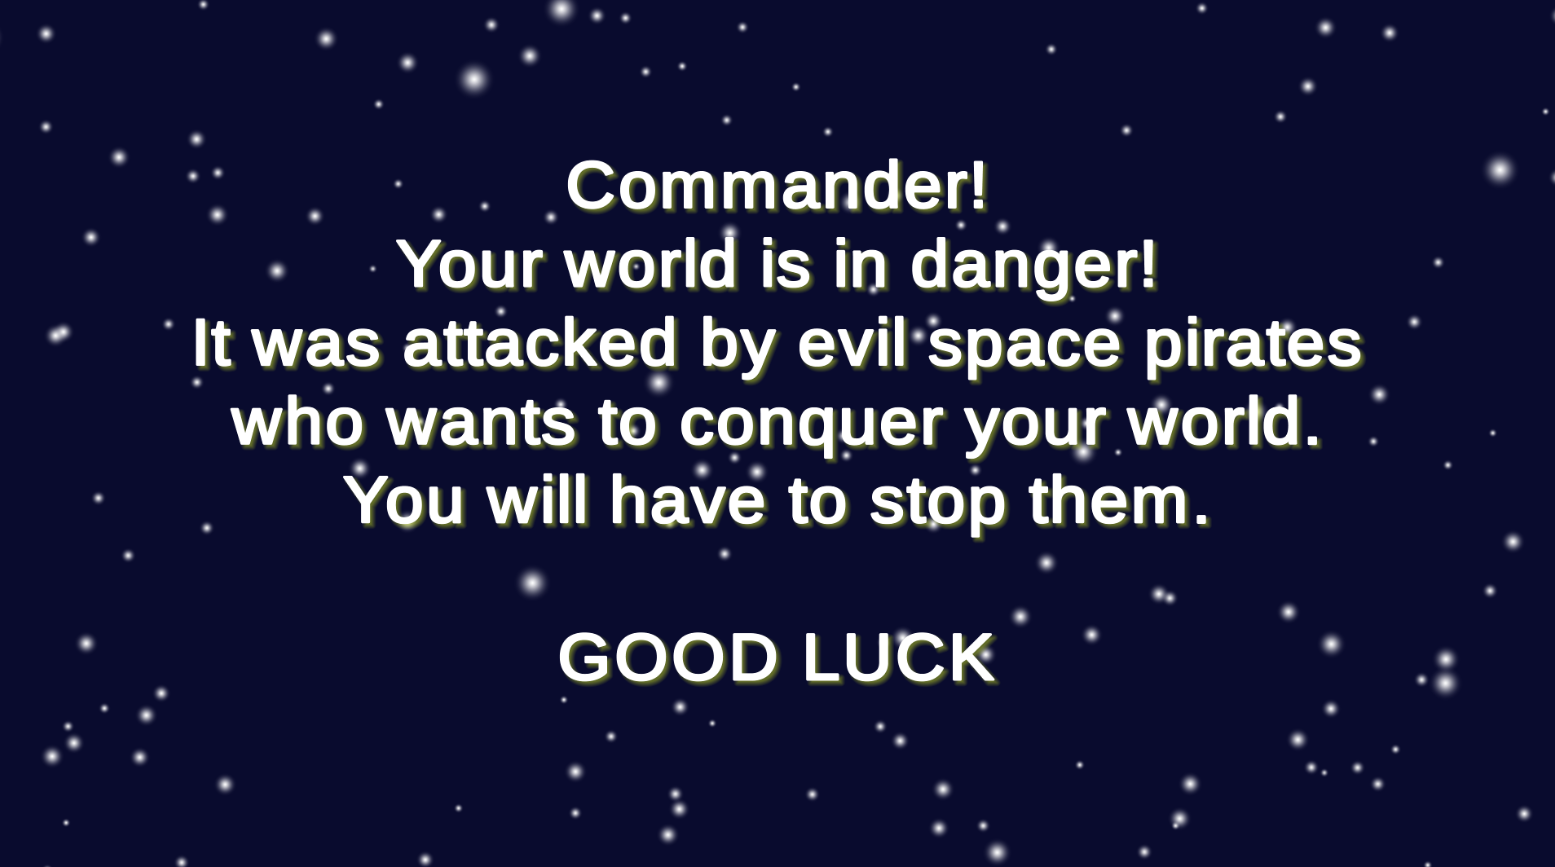
\includegraphics[width=0.9\linewidth]{images/nonaffectiveintroduction.png}
		\caption{Wprowadzenie w~wersji podstawowej}
		\label{fig:nonaffectiveintroduction}
	\end{subfigure}%
	\begin{subfigure}{0.5\textwidth}
		\centering
		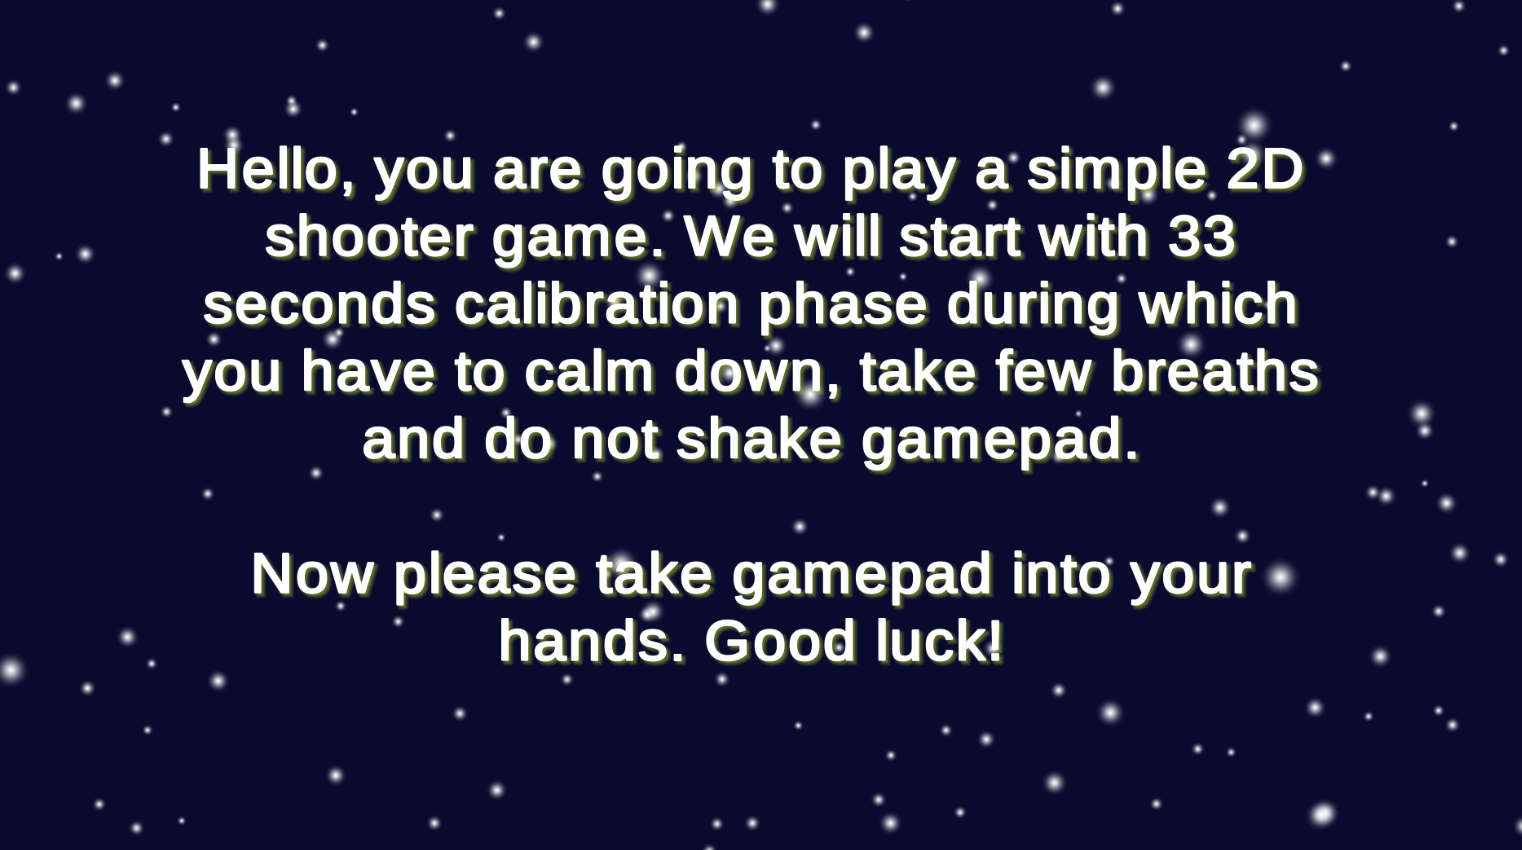
\includegraphics[width=0.9\linewidth]{images/affectiveintroduction.png}
		\caption{Wprowadzenie w~wersji afektywnej}
		\label{fig:affectiveintroduction}
	\end{subfigure}
	\caption{Ekran wprowadzenia dla obu wersji gier}
	\label{fig:introductions}
\end{figure}

Kolejnym krokiem w~integracji interfejsu było przygotowanie mechanik afektywnych, które wpływają na poszczególne elementy rozgrywki w~zależności od odczuwanych przez użytkownika emocji lub napięcia mięśni przedramienia. W~ramach skryptów odpowiadających za konkretne elementy rozgrywki przygotowane zostały funkcje, które następnie zarejestrowano jako obserwatorzy wystąpienia nowej emocji lub napięcia mięśni. Aby ułatwić interpretację poziomów \textit{valence} i~\textit{arousal} zwracanych w~ramach obiektu reprezentującego odczuwaną emocję, stworzone zostały stałe, które przypisują każdą z~par obu wartości do konkretnej emocji. Interpretacja każdej z~kombinacji została przedstawiona w~tabeli~\ref{tab:emotions}. W~ramach zaimplementowanych mechanik afektywnych można wyróżnić:
\begin{enumerate}
	\item \textbf{Aktywacja mocy specjalnej po wykryciu napięcia mięśni przedramienia}. Mechanika ta stanowi alternatywę dla uruchomienia mocy specjalnej przy pomocy przycisku na kontrolerze. Uruchomienie jej bez wyłączania akcji z~podstawowej wersji gry pozwala użytkownikowi wybrać sposób aktywacji, który jest dla niego wygodniejszy.
	\item \textbf{Aktywacja mocy specjalnej w~momencie, gdy gracz przez dłuższy czas odczuwa złość}. W~odróżnieniu od poprzedniego punktu, w~tym przypadku moc specjalna aktywowana jest niezależnie od jej dostępności w~momencie, gdy poprzednia i~aktualnie odczytana emocja to złość. 
	\item \textbf{Zmiana ilości punktów życia gracza na podstawie odczuwanych emocji}. Można wyróżnić tutaj następujące możliwości:
	\begin{itemize}
		\item Odebranie graczowi 40\% punktów życia w~przypadku odczuwania przez dłuższy czas emocji neutralnej, zmęczenia lub zrelaksowania. Taka reakcja miała na celu pobudzenie gracza do skupienia się na rozgrywce ze względu na nagłą trudną sytuację.
		\item Odebranie graczowi 20\% punktów życia w~momencie odczuwania przez dłuższy czas szczęścia lub ekscytacji. Emocje te zostały wydzielone do lżejszej wersji negatywnego efektu, aby uniknąć nadmiernego zdenerwowania gracza, ale jednocześnie wzbudzić w~nim potrzebę skupienia się na grze.
		\item Przywrócenie 10\% punktów życia w~momencie odczuwania smutku lub strachu. Efekt ten miał posłużyć jako pomoc dla gracza i~wywołanie przez to u niego pozytywnych emocji.
	\end{itemize}
	\item \textbf{Aktywacja dodatkowych fal przeciwników w~przypadku odczuwania przez gracza emocji neutralnej, zrelaksowania, zmęczenia lub szczęścia}. W~przypadku trzech pierwszych emocji mechanika ta miała na celu postawienie graczowi wyzwania. Uruchomienie jej w~momencie odczuwania szczęścia przez gracza miało na celu wywołanie u niego emocji przeciwstawnych takich jak strach czy złość.
	\item \textbf{Aktywacja i~dezaktywacja trybu trudnego gry w~zależności od odczuwanej emocji}. Mechanika ta zastępowała jej podstawową wersję opartą na częstotliwości zdobywania punktów. W~przypadku odczuwania przez gracza złości lub strachu była ona dezaktywowana, natomiast aktywacja następowała w~momencie odczuwania przez gracza emocji neutralnej, zrelaksowania lub zmęczenia.
\end{enumerate}

\begin{table}
	\centering
	\caption{Interpretacja kombinacji poziomów \textit{valence} i~\textit{arousal} jako emocje.}
	\label{tab:emotions}
	\begin{tabular}{|l|l|l|l|}
		\hline
		\diagbox[width=8em]{\textbf{Valence}}{\textbf{Arousal}}      & LOW    & MEDIUM           & HIGH          \\ \hline
		LOW    & Smutek & Złość        & Strach \\ \hline
		MEDIUM & Zmęczenie  & Emocja neutralna & Zaskoczenie     \\ \hline
		HIGH   & Zrelaksowanie & Szczęście      & Ekscytacja    \\ \hline
	\end{tabular}
\end{table}

Implementacja interfejsu do rozpoznawania emocji i~zachowań gracza umożliwiła stworzenie gry zawierającej pętlę afektywną. Aby zrealizować w~pełni założenia programowania afektywnego, każda z~mechanik zmieniała rozgrywkę w~taki sposób, aby wzbudzić w~użytkowniku inny rodzaj emocji od aktualnie odczuwanych. Przygotowany interfejs umożliwił łatwą implementację każdej z~nich bez konieczności modyfikacji oryginalnego kodu gry dzięki rejestracji funkcji uruchamianych w~momencie odczytania emocji.

\chapter{Badania}
\label{cha:badania}
\section{Procedura eksperymentu}
W jaki sposób przebiegał eksperyment 
\section{Uczestnicy}
Opis uczestników, wiek, płeć, ewentualny stan zdrowotny
\section{Analiza wyników}
Jakie emocje były odczuwane i jak często, czy uczestnicy byli zainteresowani interfejsem, działaniem samej gry, czy zauważali mechaniki w zależności od odczuwanych emocji
\chapter{Podsumowanie}
\label{cha:podsumowanie}
\section{Wnioski}
Niniejsza praca miała na celu zaprojektowanie i~przygotowanie interfejsu składającego się ze zbioru platform sprzętowych umożliwiających pomiar sygnałów fizjologicznych i~zachowań użytkownika oraz modułu programistycznego w~wybranym środowisku do tworzenia gier, którego zadaniem jest określenie stanu emocjonalnego i~zachowań użytkownika. Rozwiązanie zostało zrealizowane w~kilku etapach.

Pracę rozpoczęto od przeglądu literatury o~tematyce emocji i~programowania afektywnego. Szczególną uwagę poświęcono modelom reprezentacji stanów emocjonalnych i~pojęciu pętli afektywnej. Odwołano się także do aktualnie istniejących gier, które realizują założenia programowania afektywnego lub wykorzystują sygnały fizjologiczne do wpływania na rozgrywkę.

Kolejnym krokiem była analiza dostępnych rozwiązań w~zakresie platform sprzętowych do pomiaru sygnałów fizjologicznych, możliwych mechanizmów wnioskowania oraz narzędzi wykorzystywanych do budowy gier komputerowych. Opisane zostały wady i~zalety wyboru poszczególnych rozwiązań sprzętowych, działanie wybranych metod wnioskowania oraz możliwości kilku dostępnych darmowych silników do tworzenia gier. Podczas analizy rozwiązań sprzętowych zwrócono uwagę na wyższość urządzeń nasobnych, które oferowały wysoki komfort użytkowania, jednocześnie pozwalając na dokładny odczyt sygnałów fizjologicznych. Zwrócono także uwagę na urządzenia, które oferowały pomiary pośrednie, takie jak odczyty z~kontrolerów do gier, umożliwiające określenie stanu użytkownika.

Następnie przeprowadzone zostało przygotowanie części sprzętowej projektu. Określone zostały podstawowe założenia wymagane do spełnienia przez urządzenia wchodzące w~skład interfejsu. Najważniejszym aspektem było uzyskanie jak najdokładniejszych pomiarów, nie powodując przy tym wzrostu dyskomfortu w~czasie użytkowania. Dla każdego z~urządzeń przedstawione zostały argumenty uzasadniające ich wybór. Zwrócono uwagę na dostępne sposoby komunikacji, a~także sposób montażu każdego z~urządzeń.

Część programistyczną projektu rozpoczęto od przygotowania modelu uczenia maszynowego do rozpoznawania emocji. Wybrane zostały zbiory danych uczących, które następnie poddano wstępnemu przetworzeniu. Określono także cechy bazujące na pomiarach pracy serca oraz zbiór klas rozpoznawanych przez model, które stanowią reprezentację poszczególnych stanów emocjonalnych. Następnie przetestowano modele oparte na kilku algorytmach uczenia maszynowego i~wybrano ostatecznie klasyfikator ekstremalnych drzew losowych charakteryzujący się najwyższą skutecznością.

Ostatnią częścią przygotowaną w~ramach niniejszej pracy była implementacja głównego elementu, którym był moduł programistyczny komunikujący się z~wybranymi urządzeniami i~określający stan emocjonalny użytkownika. Równocześnie została także stworzona gra komputerowa, która wykorzystywała interfejs do obsługi zmian mechanik rozgrywki w~zależności od zachowań i~emocji gracza. 

Stworzona gra została następnie wykorzystana w~celu ewaluacji zaimplementowanego rozwiązania. Głównymi kryteriami oceny były logi emocji określonych przez interfejs oraz kwestionariusze wypełnione przez uczestników badania po jego zakończeniu. Analizując wyniki dotyczące zauważenia zmian w~rozgrywce w~wersji gry zawierającej interfejs do określania stanu emocjonalnego gracza, wygody użytkowania części sprzętowej oraz satysfakcji osób badanych z~rozgrywki można stwierdzić, że moduł stworzony w~ramach niniejszej pracy magisterskiej realizuje główny cel projektu. Taka ocena może wskazywać także na to, że wprowadzenie mechanizmów opartych o~emocje na rynek komercyjny gier komputerowych ma nadzieję spotkać się z~pozytywnym odzewem branży oraz graczy.

\section{Propozycje przyszłych prac}
Choć stworzony interfejs spełnia wymagania określone w~celach niniejszej pracy magisterskiej, możliwe jest rozszerzenie poszczególnych jego elementów. Można rozważyć dodanie nowych urządzeń, pozwalających na pobieranie innych sygnałów fizjologicznych, takich jak reakcja elektrodermalna, czy pomiary zwracane przez elektroencefalograf. Ponieważ struktura interfejsu jest modułowa, rozwiązanie to wymagałoby przygotowania skryptów do komunikacji i~interpretacji nowych sygnałów. 

Elementem wartym dopracowania jest także model rozpoznający emocje. Poprzez wprowadzenie nowych sygnałów możliwe byłoby przygotowanie zbioru o~wyższej skuteczności. Jednocześnie rozwiązaniem wartym uwagi jest wykorzystanie sieci neuronowej zamiast klasyfikatorów. Możliwe, że taka zmiana podejścia podczas projektowania modelu do rozpoznawania emocji pozwoli uzyskać rezultaty znacznie wyższe od uzyskanych w~ramach niniejszej pracy magisterskiej. Jednocześnie w~ramach modelu mogłyby też zostać uwzględnione odczyty bazowe zbierane w~trakcie fazy kalibracji. Pozwoliłoby to na porównanie sygnałów fizjologicznych zbieranych w~czasie gry z~wartościami spoczynkowymi. 

Ponadto, przygotowany moduł zawiera także elementy wymagające poprawy. Poza wspomnianym wcześniej modelem do rozpoznawania emocji należałoby zabezpieczyć także moment weryfikacji zwracanych emocji przez odczyty z~akcelerometru w~taki sposób, aby nie obniżał nadmiernie wartości \textit{arousal} w~przypadku gdy użytkownik nie porusza kontrolerem w~czasie gry.





% itd.
% \appendix
% \include{dodatekA}
% \include{dodatekB}
% itd.
\printbibliography

\end{document}
